\section{Analisi dei componenti}
\label{secD2:AnalisiDeiComponenti}

Nel presente capitolo viene presentata l'architettura in termini di componenti (ACI) interni al sistema definiti sulla base dei requisiti analizzati nei precedenti documenti. Viene poi adottato l'uso di Component Diagram per rappresentare l'interconnessione tra i vari componenti, identificando quindi le interfacce tra questi e verso sistemi esterni.

\subsection{DEFINIZIONE DEI COMPONENTI}
In questa sezione vengono definiti i componenti.

\begin{listaPersonale}[ACI]{}

    \elemento[Gestione creazione o modifica evento]{aci:creazioneModificaEvento}

    \textbf{Motivazione:}\\
    È stato considerato il \prettyref{D1-rf:CreazioneModificaEvento} e \todo{RF2.2.1 non esiste} ed il mock-up della schermata “Eventi” in \prettyref{D1-fe:SchermataCreaModificaEvento}.
    È stato quindi definito il componente “Gestione creazione o modifica evento” allo scopo di gestire la parte di front-end della funzionalità di creazione o modifica evento per un utente non autenticato e autenticazione.
    \textbf{Spiegazione:}\\
    Il componente gestisce l'intera procedura che l'utente non autenticato segue per creare o modificare un evento. Dopo che l'utente ha definito i campi, questo componente gestisce la creazione o modifica dell'evento secondo i campi definiti. Inoltre, questo componente gestisce la creazione o modifica evento anche per utenti autenticati, i quali possono definire dei campi aggiuntivi rispetto agli utenti non autenticati; questo componente fa in modo di fornire questi campi aggiunti agli utenti autenticati standard.


    \elemento[Gestione notifiche]{aci:gestioneNotifiche}

    \textbf{Motivazione:}\\
    Per il \prettyref{D1-rf:Notifiche} e \todo{RF6.9 inserimento calendario?}, il sistema deve permettere all'utente autenticato di creare, secondo delle impostazioni scelte dall'utente autenticato, le notifiche per gli eventi del suo calendario. Il componente “Gestione notifiche” fa in modo che questa funzionalità venga implementata.
    \textbf{Spiegazione:} Il componente gestisce la funzionalità di creazione o modifica della notifica di un evento, dopo che l'utente ha definito i campi d'impostazione della notifica.


    \elemento[Interfaccia sistema di mappe]{aci:interfaciaMappe}

    \textbf{Motivazione:}\\
    Dato il \todo{RF6.6 si intende \prettyref{D1-rf:LuogoEvento}?}, il sistema deve permettere agli utenti standard di inserire il luogo dove avviene l'evento mediante l'utilizzo di un sistema di mappe esterno, per questo motivo è stato definito il componente “Interfaccia sistema di mappe”.
    \textbf{Spiegazione:} Il componente gestisce la funzionalità data all'utente standard di interagire con un sistema esterno di mappe per definire il luogo dove avviene l'evento, gestendo l'intera procedura, dall' invio del luogo al sistema esterno di mappe alla ricezione delle coordinate di questo.


    \elemento[Gestione condivisione]{aci:gestioneCondivisione}

    \textbf{Motivazione:}\\
    Dato il \prettyref{D1-rf:InterzioneTraCalendariDiAltriUtenti} e il \prettyref{D1-rf:ImpostazioniPredefiniteCalendario} e considerando il mock-up \prettyref{D1-fe:SchermataCreaModificaEvento} “Gestione crea/modifica evento” e \prettyref{D1-fe:SchermataCreaModificaCalendario} “Gestione crea/modifica calendario”, l'utente autenticato deve poter definire a quali utenti condividere un evento o un calendario. È stato quindi definito il componente “Gestione condivisione” allo scopo di gestire questa funzionalità.
    \textbf{Spiegazione:} Il componente gestisce la condivisione di eventi e calendari, ovvero fa in modo di inviare la condivisione di eventi e calendari agli utenti definiti dall'utente autenticato standard. Il componente invia la richiesta di condivisione e sovrintende l'intera procedura di condivisione fino alla ricevuta dell'esito di condivisione.


    \elemento[Gestione campi precompilati]{aci:campiPrecompilati}

    \textbf{Motivazione:}\\
    Dato il \prettyref{D1-rf:ImpostazioniPredefiniteCalendario}, è stato definito il componente “Gestione campi precompilati”, la cui funzionalità è fornire i campi precompilati di creazione o modifica evento di un specifico calendario.
    \textbf{Spiegazione:} Ciascun calendario può avere dei campi precompilati nella creazione o modifica evento, dunque la funzione del componente “Gestione campi precompilati” è quella di gestire la ricezione e invio di questi campi precompilati in tempo di creazione o modifica evento.


    \elemento[Gestione creazione o modifica calendario]{aci:creazioneM odificaCalendario}

    \textbf{Motivazione:}\\
    Per il \prettyref{D1-rf:CondivisioneCalendario} e il \prettyref{D1-rf:ImpostazioniPredefiniteCalendario} e considerando il mock-up \prettyref{D1-fe:SchermataCreaModificaCalendario} “Gestione crea/modifica calendario”, l'utente autenticato deve poter creare e modificare i propri calendari.
    Definiamo quindi il componente “Gestione creazione modifica calendario” per permettere all'utente di avere questa funzionalità.
    \textbf{Spiegazione:} Il componente gestisce la creazione e modifica di calendari da parte dell'utente autenticato standard. Nello specifico, questo componente gestisce l'intera procedura di questa funzionalità, creando o modificando un calendario secondo dei campi definiti dall'utente autenticato. Alla fine della procedura, il componente invia una schermata d'esito dell'azione.\\
    Osserviamo che questa componente è resa disponibile anche all'utente non autenticato ma in maniera limitata, ovvero solo per la modifica del calendario principale, in quanto non può avere altri calendari oltre a questo. Questa componente gestisce anche la limitazione posta all'utente non autenticato riguardo a quali campi può avere nella “Gestione creazione o modifica calendario”.


    \elemento[Gestione Dashboard]{aci:dashboard}

    \textbf{Motivazione:}\\
    È stato considerato il \prettyref{D1-rf:UsoDelTempo} e il mock-up della schermata“Dashboard” in \prettyref{D1-fe:SchermataCreaModificaCalendario}. È stata, quindi, definita questa componente allo scopo di gestire la parte di front-end per la funzionalità di ottenere informazioni sull'uso del tempo.
    \textbf{Spiegazione:}\\
    Il componente “Dashboard” permette all'utente autenticato di ottenere delle informazioni sull'uso del tempo,  mostrando dati sulle attività dell'utente non autenticato in base ad alcuni periodi di tempo. Inoltre, il componente contiene un heatmap  il cui scopo è quello di indicare il tempo che deve essere dedicato ogni giorno per rispettare le varie deadline, le quali hanno una scadenza che va da un giorno ad un semestre.


    \elemento[Gestione eventi settimanali]{aci:eventiSettimanali}

    \textbf{Motivazione:}\\
    Per il \prettyref{D1-rf:UsoDelTempo} e il mock-up \prettyref{D1-fe:AttivitaSettimanaDashboard}, il sistema deve poter mostrare all'utente non autenticato le attività settimanali mediante l'utilizzo di un grafico a barre con cui l'utente può interagire. È stato quindi definito il componente Gestione attività settimanali allo scopo di gestire questa funzionalità.

    \textbf{Spiegazione:}\\
    Il componente “Gestione attività settimanali” fa in modo di fornire delle informazioni sulle attività settimanali all'utente non autenticato mostrando un grafico a barre. Gestisce anche le interazioni che l'utente autenticato standard può avere con tale grafico.


    \elemento[Gestione eventi giornalieri]{aci:eventiGiornalieri}

    \textbf{Motivazione:}\\
    Per il \prettyref{D1-rf:UsoDelTempo} e il mock-up \prettyref{D1-fe:AttivitaGiornoEGraficoDashboard}, il sistema deve poter mostrare all'utente non autenticato le attività giornaliere mediante l'utilizzo di un grafico a torta e una lista delle attività, con cui l'utente può interagire. È stato quindi definito il componente “Gestione attività giornaliere” per gestire questa funzionalità. Inoltre, il grafico a torta e la lista delle attività giornaliere sono sincronizzati, ovvero mostrano all'utente non autenticato i dati degli stessi eventi; dunque il componente “Gestione attività giornaliere” deve fare in modo che la sincronizzazione avvenga con successo.
    \textbf{Spiegazione:}\\
    Il componente “Gestione attività giornaliere” mostra un grafico a torta e una lista delle attività giornaliere, inoltre gestisce la sincronizzazione tra i due grafici: infatti il componente permette all'utente di interagire con la lista di attività giornaliere, modificandolo, e di conseguenza “Gestione attività giornaliere” deve modificare il grafico a torta.


    \elemento[Gestione impostazioni account]{aci:impostazioniAccount}

    \textbf{Motivazione:}\\
    Dato il \prettyref{D1-rf:ImpostazioniAccount}, il sistema deve permettere all'utente autenticato di modificare le impostazioni del proprio account. Per questo motivo è stato definito il componente “Gestione impostazioni account”.
    \textbf{Spiegazione:}\\
    Il componente “Gestione impostazioni account” permette all'utente autenticato di modificare e salvare le modifiche fatte al suo account.
    “Gestione impostazioni account” fornisce una schermata d'esito per indicare il salvataggio delle modifiche, ogni volta che l'utente va a salvare le sue modifiche.


    \elemento[Gestione modifica password]{aci:modificaPassword}

    \textbf{Motivazione:}\\
    Per il \prettyref{D1-rf:RecuperoPassword}, il sistema deve rendere disponibile all'utente standard la possibilità di modificare la password. Per questo motivo è stato definito il componente “Gestione modifica password”.
    \textbf{Spiegazione:}\\
    Il componente “Gestione modifica password” implementa la funzionalità modifica della password per un utente autenticato standard. “Gestione modifica password”, dopo aver ricevuto la nuova password, la manda ad Auth0 grazie all'interfaccia “Interfaccia API Auth0”. Alla fine dell'operazione, il componente “Gestione modifica password” manderà una schermata per mostrare l'esito dell'operazione di modifica password.


    \elemento[Interfaccia management API Auth0]{aci:APIAuth0}

    \textbf{Motivazione:}\\
    Dato il \prettyref{D1-be:Autenticazione}, il componente “Interfaccia API Auth0” serve per interfacciarsi con Auth0 quando si modifica la password del proprio account (\prettyref{D1-rf:ImpostazioniAccount}). Il sistema deve interfacciarsi con Auth0, in quanto sistema esterno che gestisce le procedure di accesso e registrazione al sito, salvando nel suo sistema le credenziali di ciascun utente autenticato.
    \textbf{Spiegazione:}\\
    Il componente, dopo aver valutato che la nuova password rispetti i criteri minimi di sicurezza, aggiorna la password nel database credenziali presente in Auth0 tramite le rest api di Auth0 management.


    \elemento[Gestione utilizzo Google Calendar]{aci:googleCalendar}

    \textbf{Motivazione:}\\
    Per rispettare il \prettyref{D1-rf:GoogleCalendar}, il sistema deve permettere all'utente autenticato standard di interagire con Google Calendar, definendo il metodo di utilizzo. Dunque, è stato definito il componente “Gestione utilizzo Google Calendar” per gestire questa funzionalità.
    \textbf{Spiegazione:}\\
    Il componente “Gestione utilizzo Google Calendar” implementa la funzionalità di interazione tra la piattaforma PlanIt e l'applicazione Google Calendar. All'utente autenticato standard vengono mostrate due opzioni con cui può interagire con Google Calendar, ovvero:
    \begin{itemize}
        \item importare ed esportare manualmente gli eventi e calendari;
        \item sincronizzazione automatica degli eventi e calendari.
    \end{itemize}
    L'utente autenticato standard decide quale metodo di interazione utilizzare in base alle proprie preferenze.


    \elemento[Gestione importazione ed esportazione attraverso file]{aci:importazioneEsportazioneFile}

    \textbf{Motivazione:}\\
    Dato il \prettyref{D1-rf:ImportazioneEsportazioneManualmenteGoogleCalendar}, l'interazione con Google Calendar può essere fatta mediante un utilizzo manuale, per questo motivo è stato definito il componente “Gestione import/export attraverso file” che gestisce questa funzionalità.
    \textbf{Spiegazione:}\\
    Il componente “Gestione import/export attraverso file” gestisce l'interazione manuale di Google Calendar. Ovvero, il componente fornisce il file di esportazione del proprio calendario o di un evento, i quali possono essere caricati direttamente su Google Calendar. Allo stesso modo, questo componente può gestire file calendari ed eventi ricevuti da Google Calendar. Tutte le azioni che avvengono in questo componente sono scandite da delle schermate d'esito che avvisano l'utente riguardo al completamento o meno dell'azione richiesta.


    \elemento[Gestione sincronizzazione]{aci:importazioneEsportazioneAutomatica}

    \textbf{Motivazione:}\\
    Dato il \prettyref{D1-rf:ImportazioneEsportazioneAutomaticamenteGoogleCalendar}, l'interazione con Google Calendar può esser fatta mediante un utilizzo automatico, per questo motivo è stato definito il componente “Gestione sincronizzazione” che gestisce questa funzionalità.
    \textbf{Spiegazione:}\\
    Il componente “Gestione sincronizzazione” gestisce l'interazione automatica di Google Calendar. Ovvero, il componente richiede una sincronizzazione con l'account Google dell'utente autenticato standard. Una volta che l'utente inserirà delle credenziali corrette di Google, avverrà la sincronizzazione tra la piattaforma PlanIt e Google Calendar: ogni volta che verrà aggiunto un evento o un calendario su Google Calendar, questo verrà aggiunto anche su PlanIt, e viceversa. L'azione di richiesta sincronizzazione account Google fa ottenere all'utente anche una schermata di esito, indicante se la sincronizzazione è avvenuta con successo o meno.


    \elemento[Gestione visualizzazione calendari ed eventi]{aci:visualizzazioneCalendariEventi}

    \textbf{Motivazione:}\\
    È stato considerato il \prettyref{D1-rf:InserimentoAutomaticoCalendario} ed il mock-up  “Schermata principale” in \prettyref{D1-fe:SchermataPrincipale}.
    È stato quindi definito il componente “Gestione visualizzazione calendari e eventi” allo scopo di gestire la parte di front-end della funzionalità di visualizzazione degli eventi e calendari dell'utente non autenticato.
    \textbf{Spiegazione:}\\
    Il componente “Gestione visualizzazione calendari e eventi” gestisce le funzionalità di visualizzazione degli eventi del calendario. L'utente non autenticato, infatti, grazie a questa componente, visualizza il calendario e i suoi eventi nella pagina “Calendario”, secondo dei criteri da lui definiti.


    \elemento[Gestione filtri calendari]{aci:filtroCalendari}

    \textbf{Motivazione:}\\
    Dato il \prettyref{D1-rf:CondivisioneCalendario} e il mock-up “Gestione principale” in \prettyref{D1-fe:SchermataPrincipaleCalendario}, è stato quindi definito “Gestione filtri calendari” allo scopo di gestire la visualizzazione della lista di tutti i calendari dell'utente non autenticato e di imporre dei filtri per la visualizzazione di questi nella schermata “Calendario”.
    \textbf{Spiegazione:}\\
    Il componente “Gestione calendari personali” gestisce la visualizzazione della lista di tutti i calendari dell'utente non autenticato, sia quelli personali che condivisi con altri utenti, nel caso si trattasse di un utente autenticato standard. Grazie a questa componente, l'utente ha la possibilità di filtrare questi calendari, in modo tale che nella pagina di “Calendario” siano presenti solo gli eventi dei calendari che si preferisce.


    \elemento[Gestione filtro impegni]{aci:}

    \textbf{Motivazione:}\\
    Per il \prettyref{D1-rf:Filtro}, è stato definito il componente “Gestione filtro impegni” per permettere all'utente non autenticato di visualizzare degli eventi secondo dei criteri da lui definiti.
    \textbf{Spiegazione:}\\
    Il componente “Gestione filtro impegni” permette all'utente non autenticato di visualizzare degli eventi secondo dei criteri da lui definiti. I criteri mostrati da “Gestione filtro impegni”, che possono essere definiti per la ricerca degli eventi, sono:
    \begin{itemize}
        \item titolo evento con corrispondenza totale o parziale;
        \item data evento;
        \item priorità evento;
        \item persone incluse nell'evento, questa funzionalità, ricordiamo, è disponibile solo per gli utenti autenticati standard. Il componente gestirà la presenza o meno di questo criterio in base alla tipologia dell'account dell'utente.
    \end{itemize}
    Una volta che l'utente non autenticato definirà i valori di questi criteri, il componente mostrerà una lista degli eventi che seguono i criteri definiti dall'utente non autenticato.


    \elemento[Gestione Attività]{aci:gestioneAttivita}

    \textbf{Motivazione:}\\
    Dato il \prettyref{D1-rf:ResocontoGiornata} e il mock-up “Schermata Attività” in \prettyref{D1-fe:SchermataAttivita}, è stato quindi definito “Gestione attività” allo scopo di permettere all'utente autenticato standard di visualizzare un resoconto delle attività programmate per quella giornata avendo la possibilità di comunicare al sistema il completamento o meno delle attività, oppure anche l'eliminazione di tale evento.
    \textbf{Spiegazione:}\\
    Il componente “Gestione attività”, mostrando la lista di attività della giornata, dà la possibilità all'utente autenticato standard di indicare il completamento o meno delle attività, oppure anche l'eliminazione di tale attività. Tutte le azioni che vengono fatte dall'utente autenticato standard sono completate con l'invio della segnalazione da parte del sistema, in modo tale che l'utente autenticato standard sia avvisato riguardo all'esito della sua azione.


    \elemento[Gestione mostra informazioni evento]{aci:mostraInformazioni}

    \textbf{Motivazione:}\\
    Per il \prettyref{D1-rf:InserimentoAutomaticoCalendario}, il sistema deve permettere all'utente non autenticato di visualizzare le informazioni di un evento, presente nel calendario, una volta che viene selezionato. Per questo motivo, è stato definito il componente “Gestione mostra informazioni evento” che gestisce questa funzionalità.
    \textbf{Spiegazione:}\\
    Il componente “Gestione mostra informazioni evento” mostra le informazioni di un evento, presente in un calendario, definito dall'utente non autenticato. Le informazioni che vengono mostrate sono quelle presenti nella creazione evento (\prettyref{D1-rf:CreazioneModificaEvento}).


    \elemento[Gestione Homepage]{aci:homepage}

    \textbf{Motivazione:}\\
    Dato il \prettyref{D1-rf:AccessoRegistrazione}, il sistema deve dare la possibilità di accedere al sito autenticazione oppure utilizzando la modalità demo del sito. È stato, quindi, definito il componente Homepage che gestisce questa funzionalità, ovvero la scelta tra entrare nel sito autenticandosi o utilizzando la modalità demo.
    \textbf{Spiegazione:}\\
    Il componente “Homepage” mostra le due scelte con cui si può entrare nel sito, o mediante la modalità demo del sito, che non richiede l'autenticazione, o la modalità completa, che richiede l'autenticazione. Una volta che il cliente della piattaforma decide quale modalità del sito utilizzare, il componente “Homepage” riceve la sua risposta e a questo punto manda le richieste ad altre componenti che implementano l'accesso richiesto dal cliente.


    \elemento[Gestione metodo di pagamento]{aci:metodoDiPagamento}
    \textbf{Motivazione:}\\
    Dato il \prettyref{D1-rf:PagamentoUtentePremium}, il sistema deve permettere ad un utente autenticato di scegliere con che metodo di pagamento acquistare l'abbonamento premium
    \textbf{Spiegazione:}\\
    Il componente deve gestire la procedura con il quale l'utente può cambiare metodo di pagamento utilizzato per l'acconto mensile del costo del piano premium.


    \elemento[Gestione abbonamento]{aci:abbonamento}

    \textbf{Motivazione:}\\
    L'utente deve poter sottoscrivere un abbonamento al sito, che lo porta ad ottenere un account premium (\prettyref{D1-rf:ImpostazioniAccount}). Per questo motivo è stato definito questo componente “Gestione abbonamento”.
    \textbf{Spiegazione:}\\
    Il componente permette all'utente di passare ad un account premium con la sottoscrizione al relativo abbonamento o permette all'utente di terminare il piano premium rinunciando ai vantaggi da esso forniti


    \elemento[Interfaccia PayPal]{aci:PayPal}

    \textbf{Motivazione:}\\
    Il sito deve dare la possibilità all'utente di effettuare l'acquista dell'abbonamento utilizzando il servizio esterno di pagamenti di paypal.
    \textbf{Spiegazione:}\\
    Il componente reindirizza l'utente sulla pagina di pagamento di paypal dove può acquistare l'abbonamento e salva i dati, quali: email dell'account paypal, username account paypal, stato pagamento, del pagamento a transazione finalizzata.


    \elemento[Interfaccia Stripe]{aci:Stripe}
    \textbf{Motivazione:}\\
    Il sito deve dare la possibilità all'utente di effettuare l'acquista dell'abbonamento utilizzando il servizio esterno di pagamenti di stripe
    \textbf{Spiegazione:}\\
    Il componente reindirizza l'utente sulla pagina di pagamento di stripe dove può acquistare l'abbonamento e salva i dati, quali: user payment token, stato pagamento, del pagamento a transazione finalizzata.


    \elemento[Gestione chiamate MongoDB]{aci:mongoDB}

    \textbf{Motivazione:}\\
    Per rispettare il \todo{RF1 (creazione/modifica evento), RF6(pagamento)},  \prettyref{D1-rf:PagamentoUtentePremium}, \prettyref{D1-rf:CondivisioneCalendario}, \prettyref{D1-rf:Notifiche}, \prettyref{D1-rf:GoogleCalendar} e \prettyref{D1-rf:ImpostazioniPredefiniteCalendario} e \prettyref{D1-rf:ImpostazioniAccount} dobbiamo salvare le impostazioni delle funzionalità di tali requisiti nel database MongoDB, per questo motivo è stato definito questo componente “Gestione chiamate MongoDB”, il quale avrà lo scopo, infatti di interfacciarsi, con MongoDB.

    \textbf{Spiegazione:}\\
    Il componente deve permettere di fare chiamate per leggere i dati dal database esterno MongoDB in modo ottimizzato e resistente ai fallimenti: questo componente deve permettere di accedere a contenuti già richiesto in modo veloce tramite un cache, dove vengono salvati gli ultimi dati letti. In caso di fallimento dell'invio dei dati da parte del server, il componente deve chiederli nuovamente dopo un breve intervallo di tempo che cresce in modo incrementale per ogni richiesta che non arriva al database.


    \elemento[Gestione account]{aci:gestioneAccount}

    \textbf{Motivazione:}\\
    Il sistema deve gestire la richiesta di autenticazione (\prettyref{D1-rf:AccessoRegistrazione}) e salvare i dati account dell'utente autenticato (\prettyref{D1-rf:ImpostazioniAccount}), per questo motivo è stato definito questo componente.

    \textbf{Spiegazione:}\\
    Il componente deve gestire la procedura di richiesta di autenticazione. Quando avvenuta, deve richiedere al database esterno i dati aggiuntivi del relativo utente quali: tipologia di abbonamento, sistema di mappe predefinito, username, sistema di pagamento predefinito, informazioni riguardanti al pagamento tramite PayPal, informazioni riguardanti al pagamento tramite Stripe, numero di ore sonno e le impostazioni della integrazione con Google Calendar. Tali dati devono essere forniti ai vari componenti che ne necessitano l'uso


    \elemento[Interfaccia Auth0]{aci:Auth0}

    \textbf{Motivazione:}\\
    Il sistema deve permettere all'utente di autenticarsi con l'uso di credenziali o con accesso mediante software esterni quali Google (\prettyref{D1-rf:MetodiAutenticazione}), per questo motivo è stato definito questo componente. Inoltre, questo componente gestisce anche il recupero della password.

    \textbf{Spiegazione:}\\
    Il componente deve gestire il reindirizzamento dell'utente sulla pagina di accesso provvista da Auth0. Ad accesso avvenuto deve fare accedere l'utente alla piattaforma. Inoltre, questa interfaccia gestisce la richiesta da parte dell'utente non autenticato del recupero password, inviando una richiesta ad Auth0 dell'invio dell'email di recupero. Dopo tale richiesta, Auth0 gestirà completamente la procedura di recupero password.


    \elemento[Interfaccia Iubenda]{aci:Iubenda}

    \textbf{Motivazione:}\\
    Il sistema deve visualizzare ad un utente che visita il sistema l'informativa sull'utilizzo dei cookie e sulle relative policy (\prettyref{D1-rnf:Privacy} e \prettyref{D1-rnf:Cookie}), quindi è stato definito questo componente.

    \textbf{Spiegazione:}\\
    Il componente deve mostrare il banner che presenta all'utente la scelta sul autorizzare l'utilizzo dei cookie da parte del sistema e salvare la risposta dell'utente, inoltre nello stesso banner deve presentare il link alla pagina di descrizione delle policy del sistema.

    \todo{Nel documenti originale manca il 4.1.30, errore?}

    \elemento[Interfaccia Cloudflare]{aci:CloudFlare}
    \textbf{Motivazione:}\\
    Il componente deve prevenire attacchi DDOS e filtrare il traffico delle richieste al sistema per rispettare \prettyref{D1-rnf:DDOSSicurezza}.

    \textbf{Spiegazione:}\\
    Il componente deve analizzare tutto il traffico proveniente dall'esterno che richiede il sistema e filtrarlo bloccando il traffico a tutti gli attori malevoli.
\end{listaPersonale}






































\subsection{DIAGRAMMA DEI COMPONENTI}

\begin{center}
    
    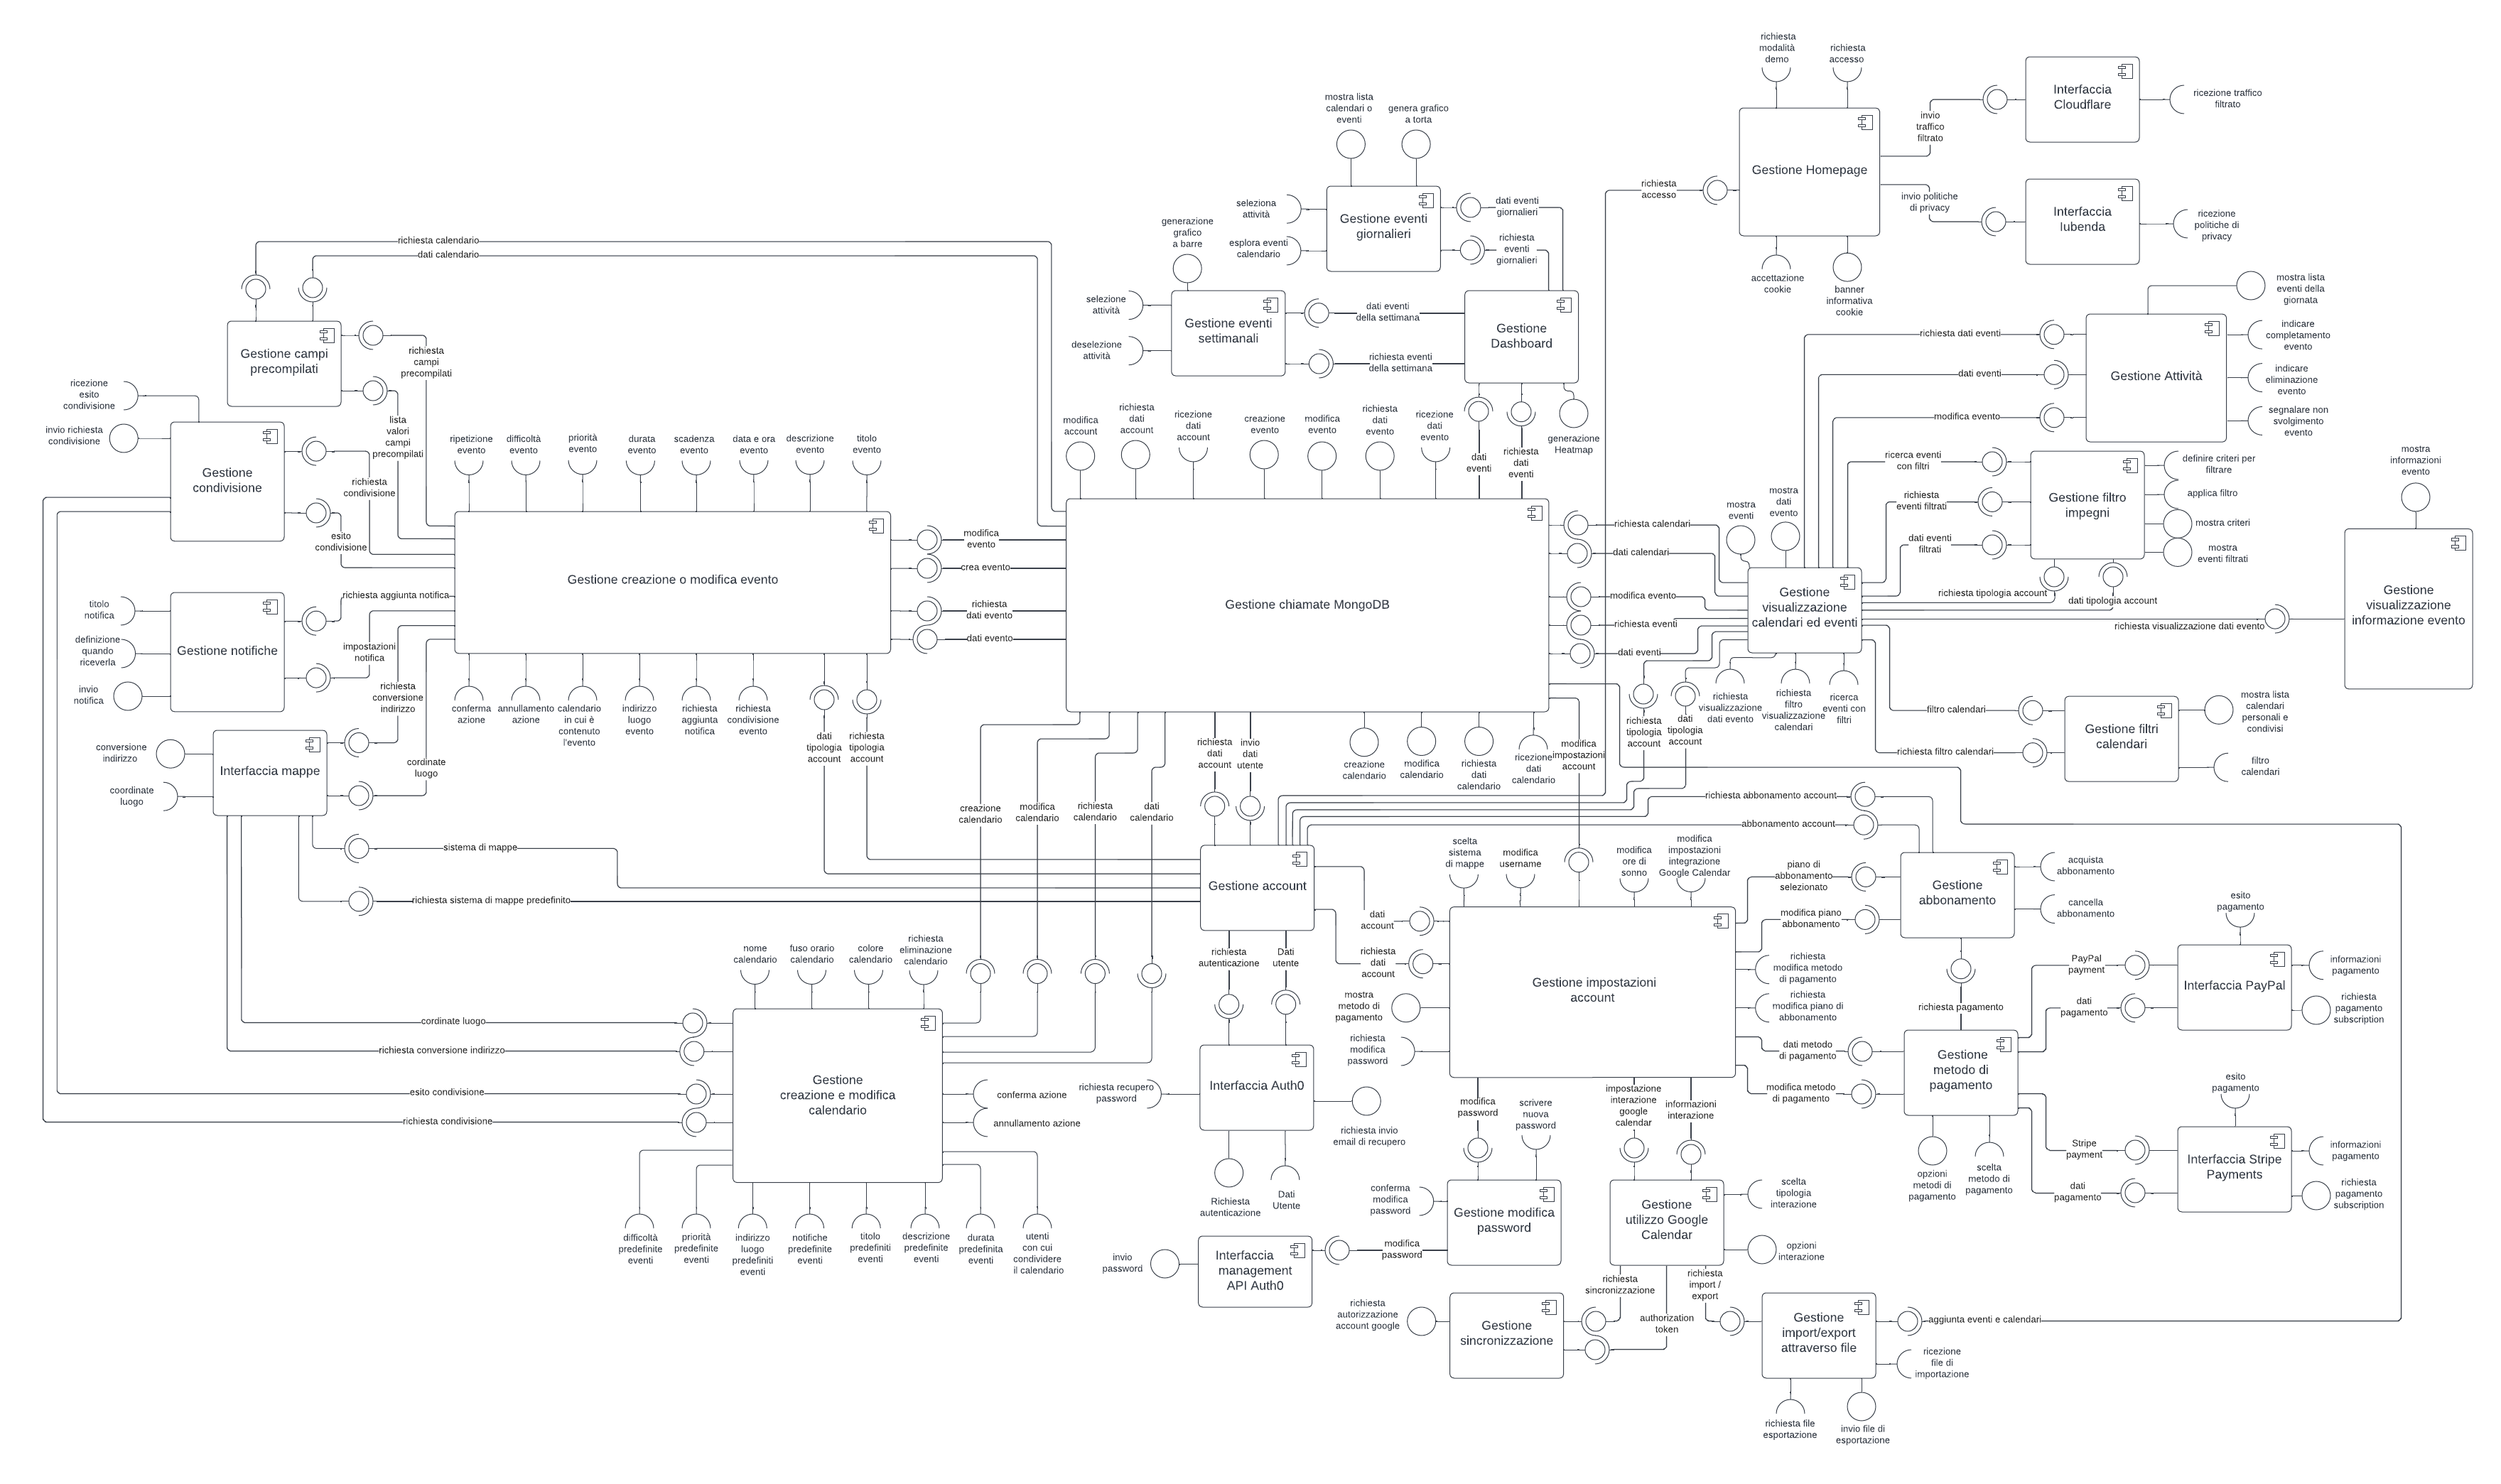
\includegraphics[width=1\textwidth,height=0.4\textheight]{img/Diagrammi/Componenti/Diagramma_dei_componenti.png}
    Questa figura mostra tutto il diagramma dei componenti del sito PlanIt.
\end{center}
\begin{center}
    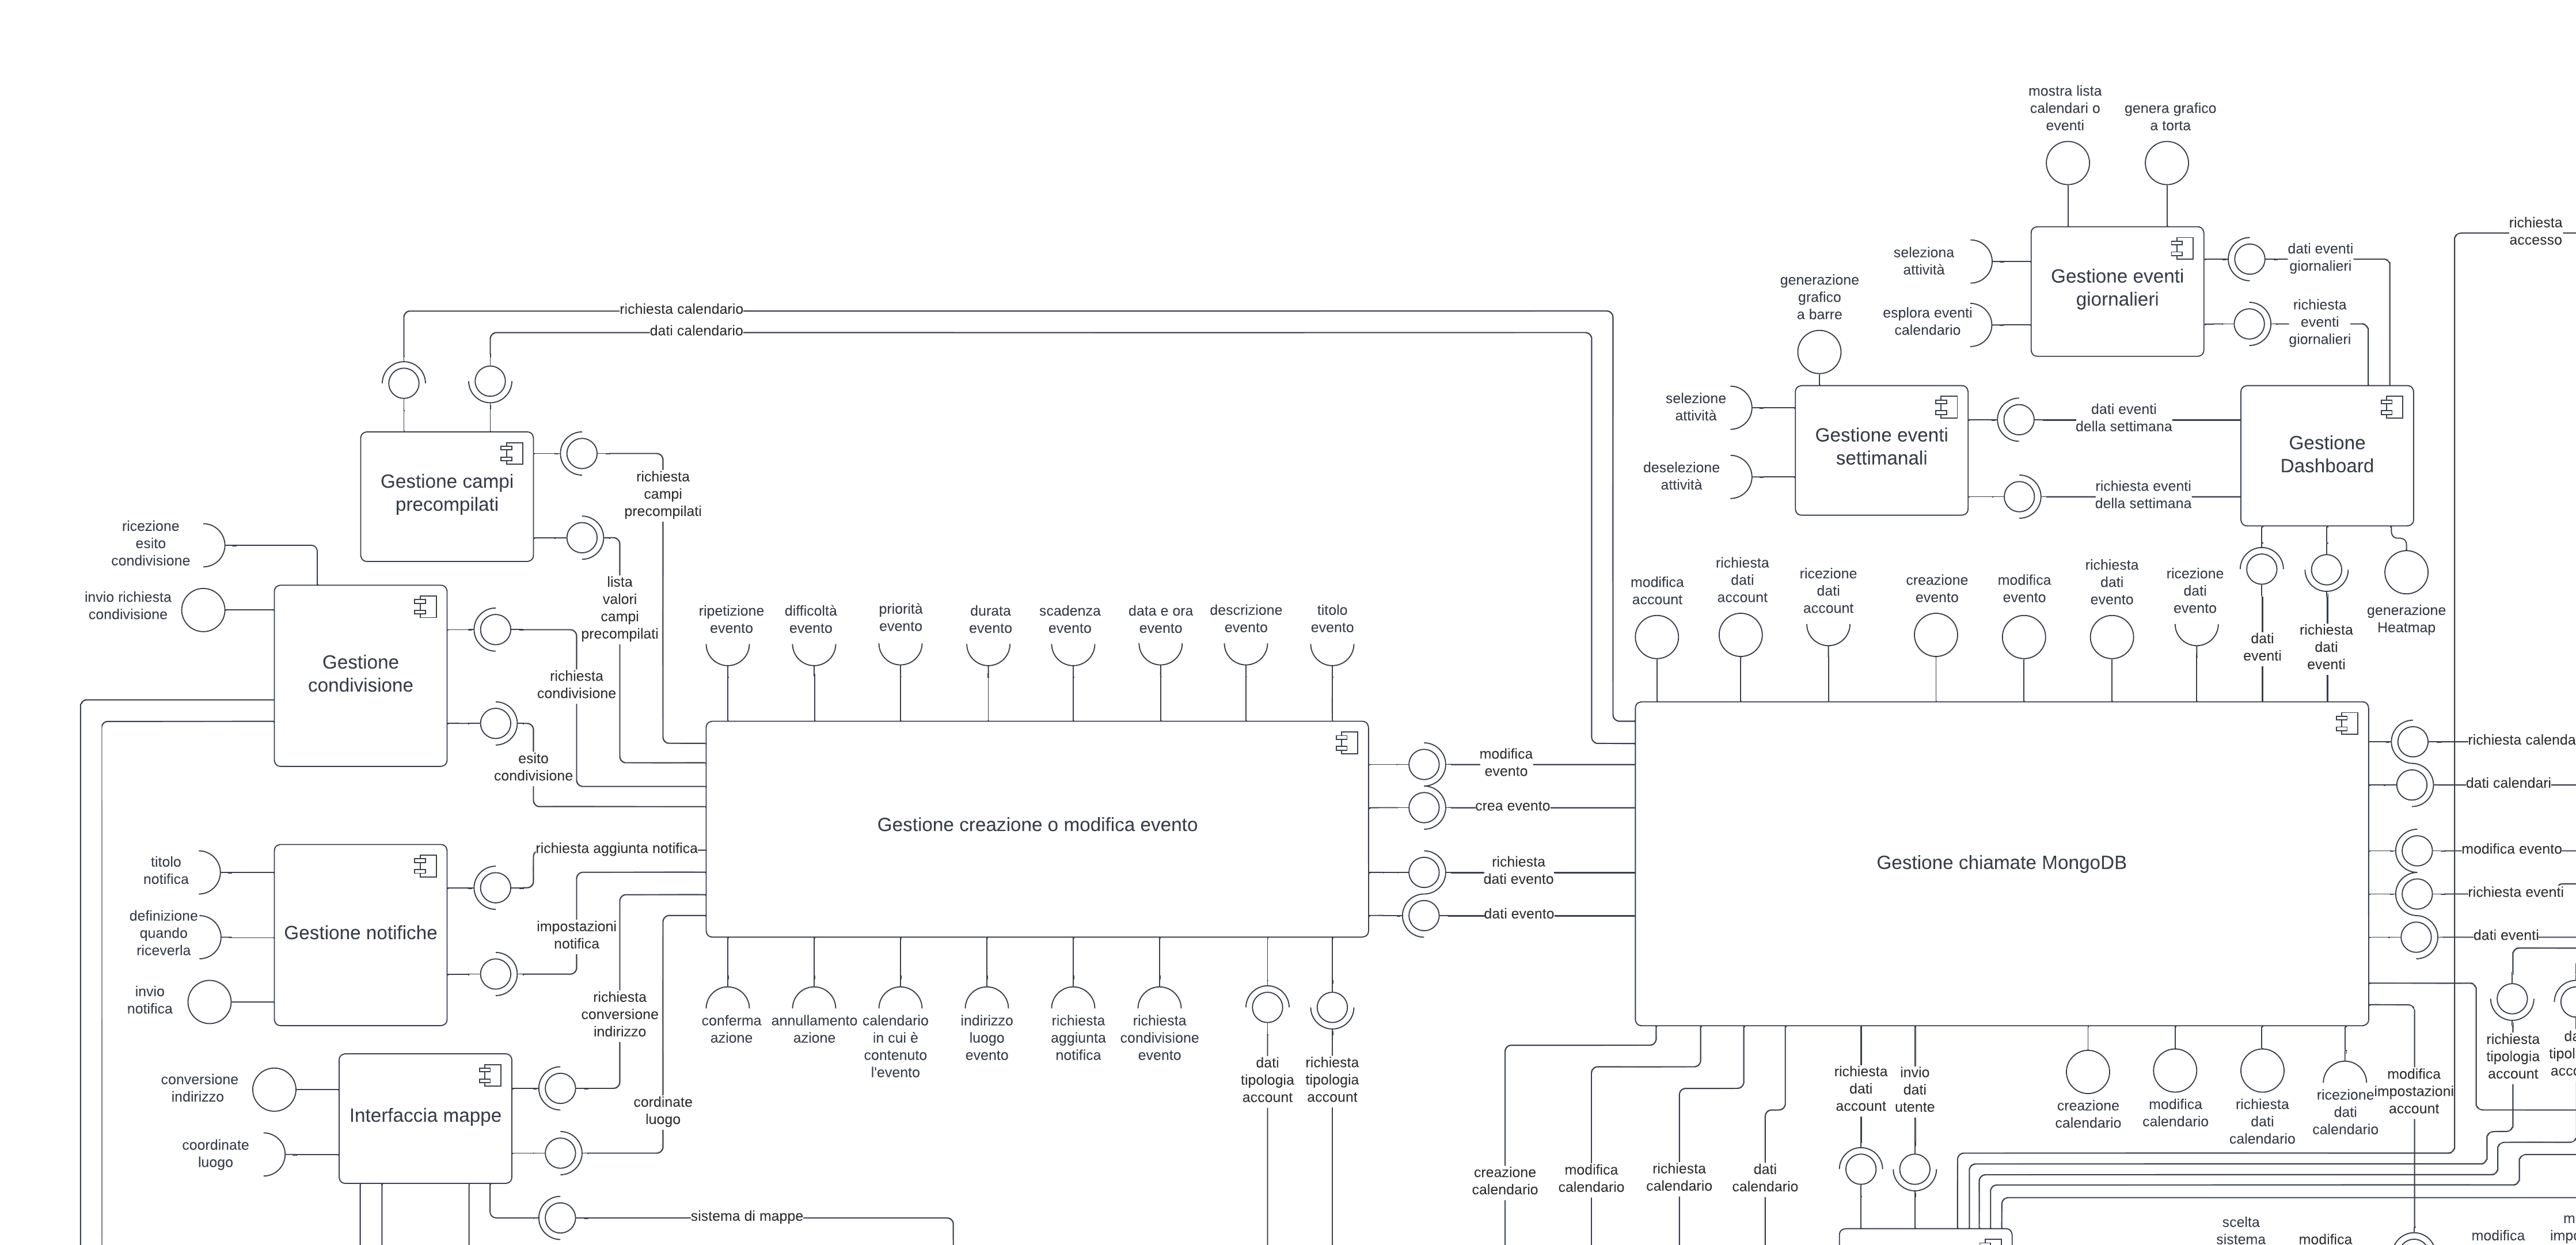
\includegraphics[width=1\textwidth,height=0.3\textheight]{img/Diagrammi/Componenti/P1_Diagramma_dei_componenti.png}
    Questa figura mostra tutto il quarto in alto a sinistra del diagramma dei componenti del sito PlanIt.
\end{center}
\begin{center}
    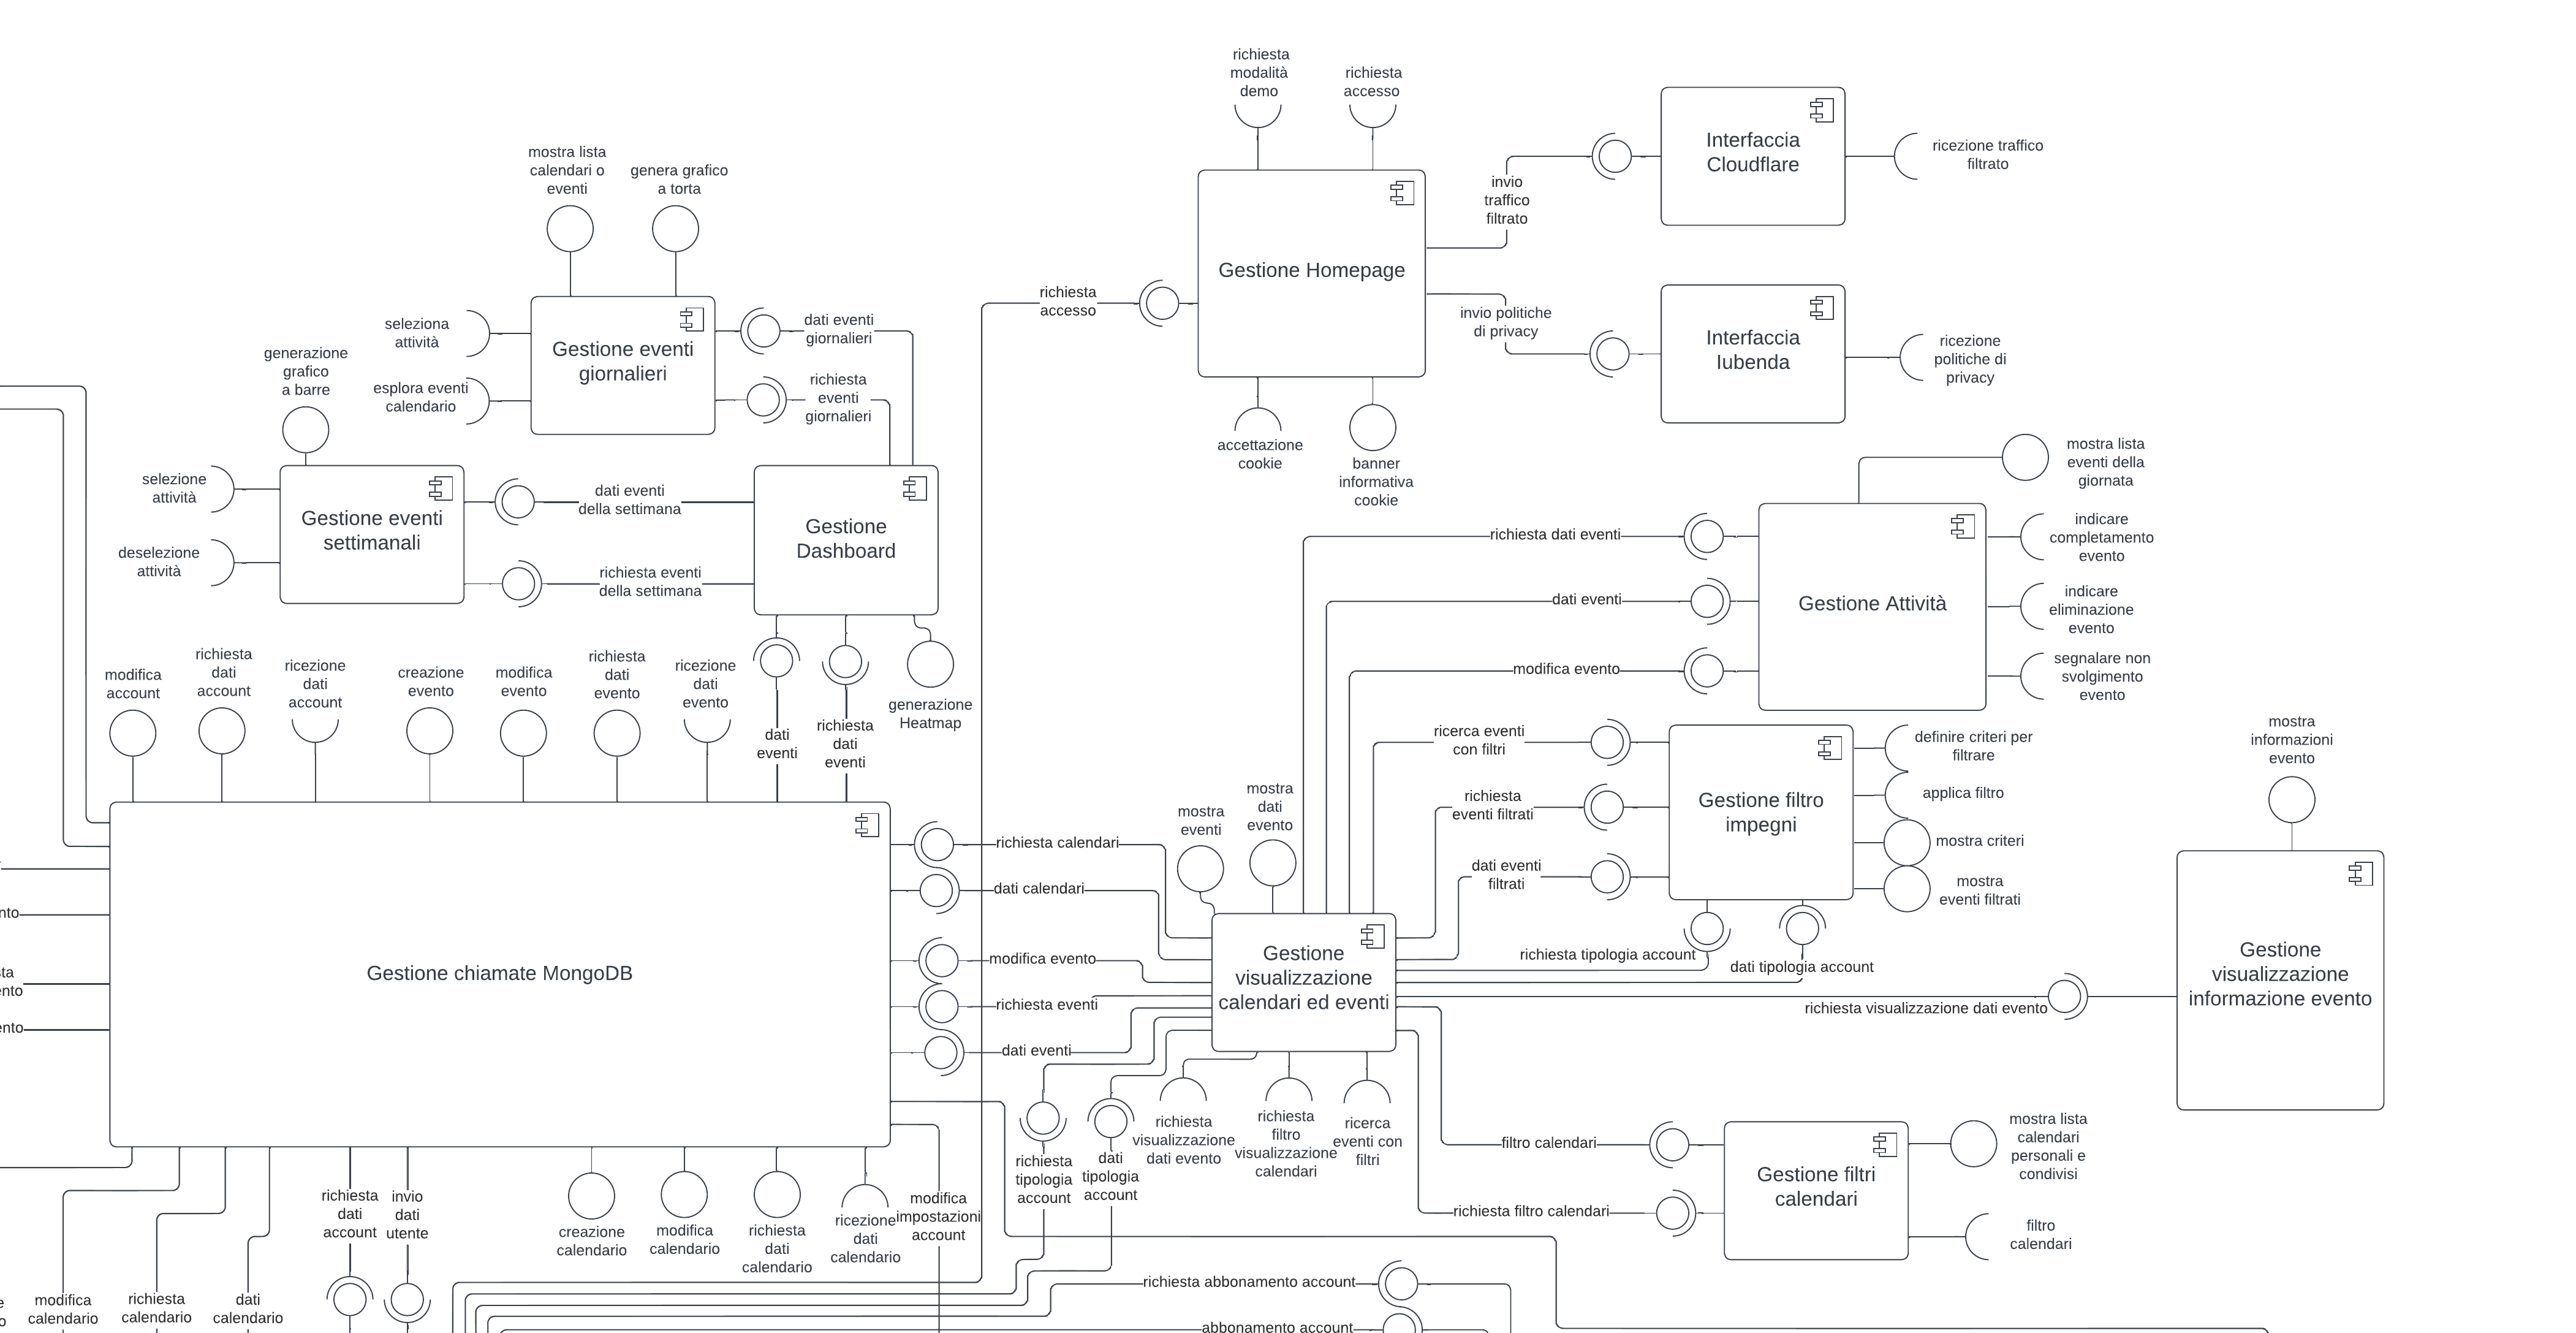
\includegraphics[width=1\textwidth,height=0.3\textheight]{img/Diagrammi/Componenti/P2_Diagramma_dei_componenti.png}
    Questa figura mostra tutto il quarto in alto a destra del diagramma dei componenti del sito PlanIt.
\end{center}
\begin{center}
    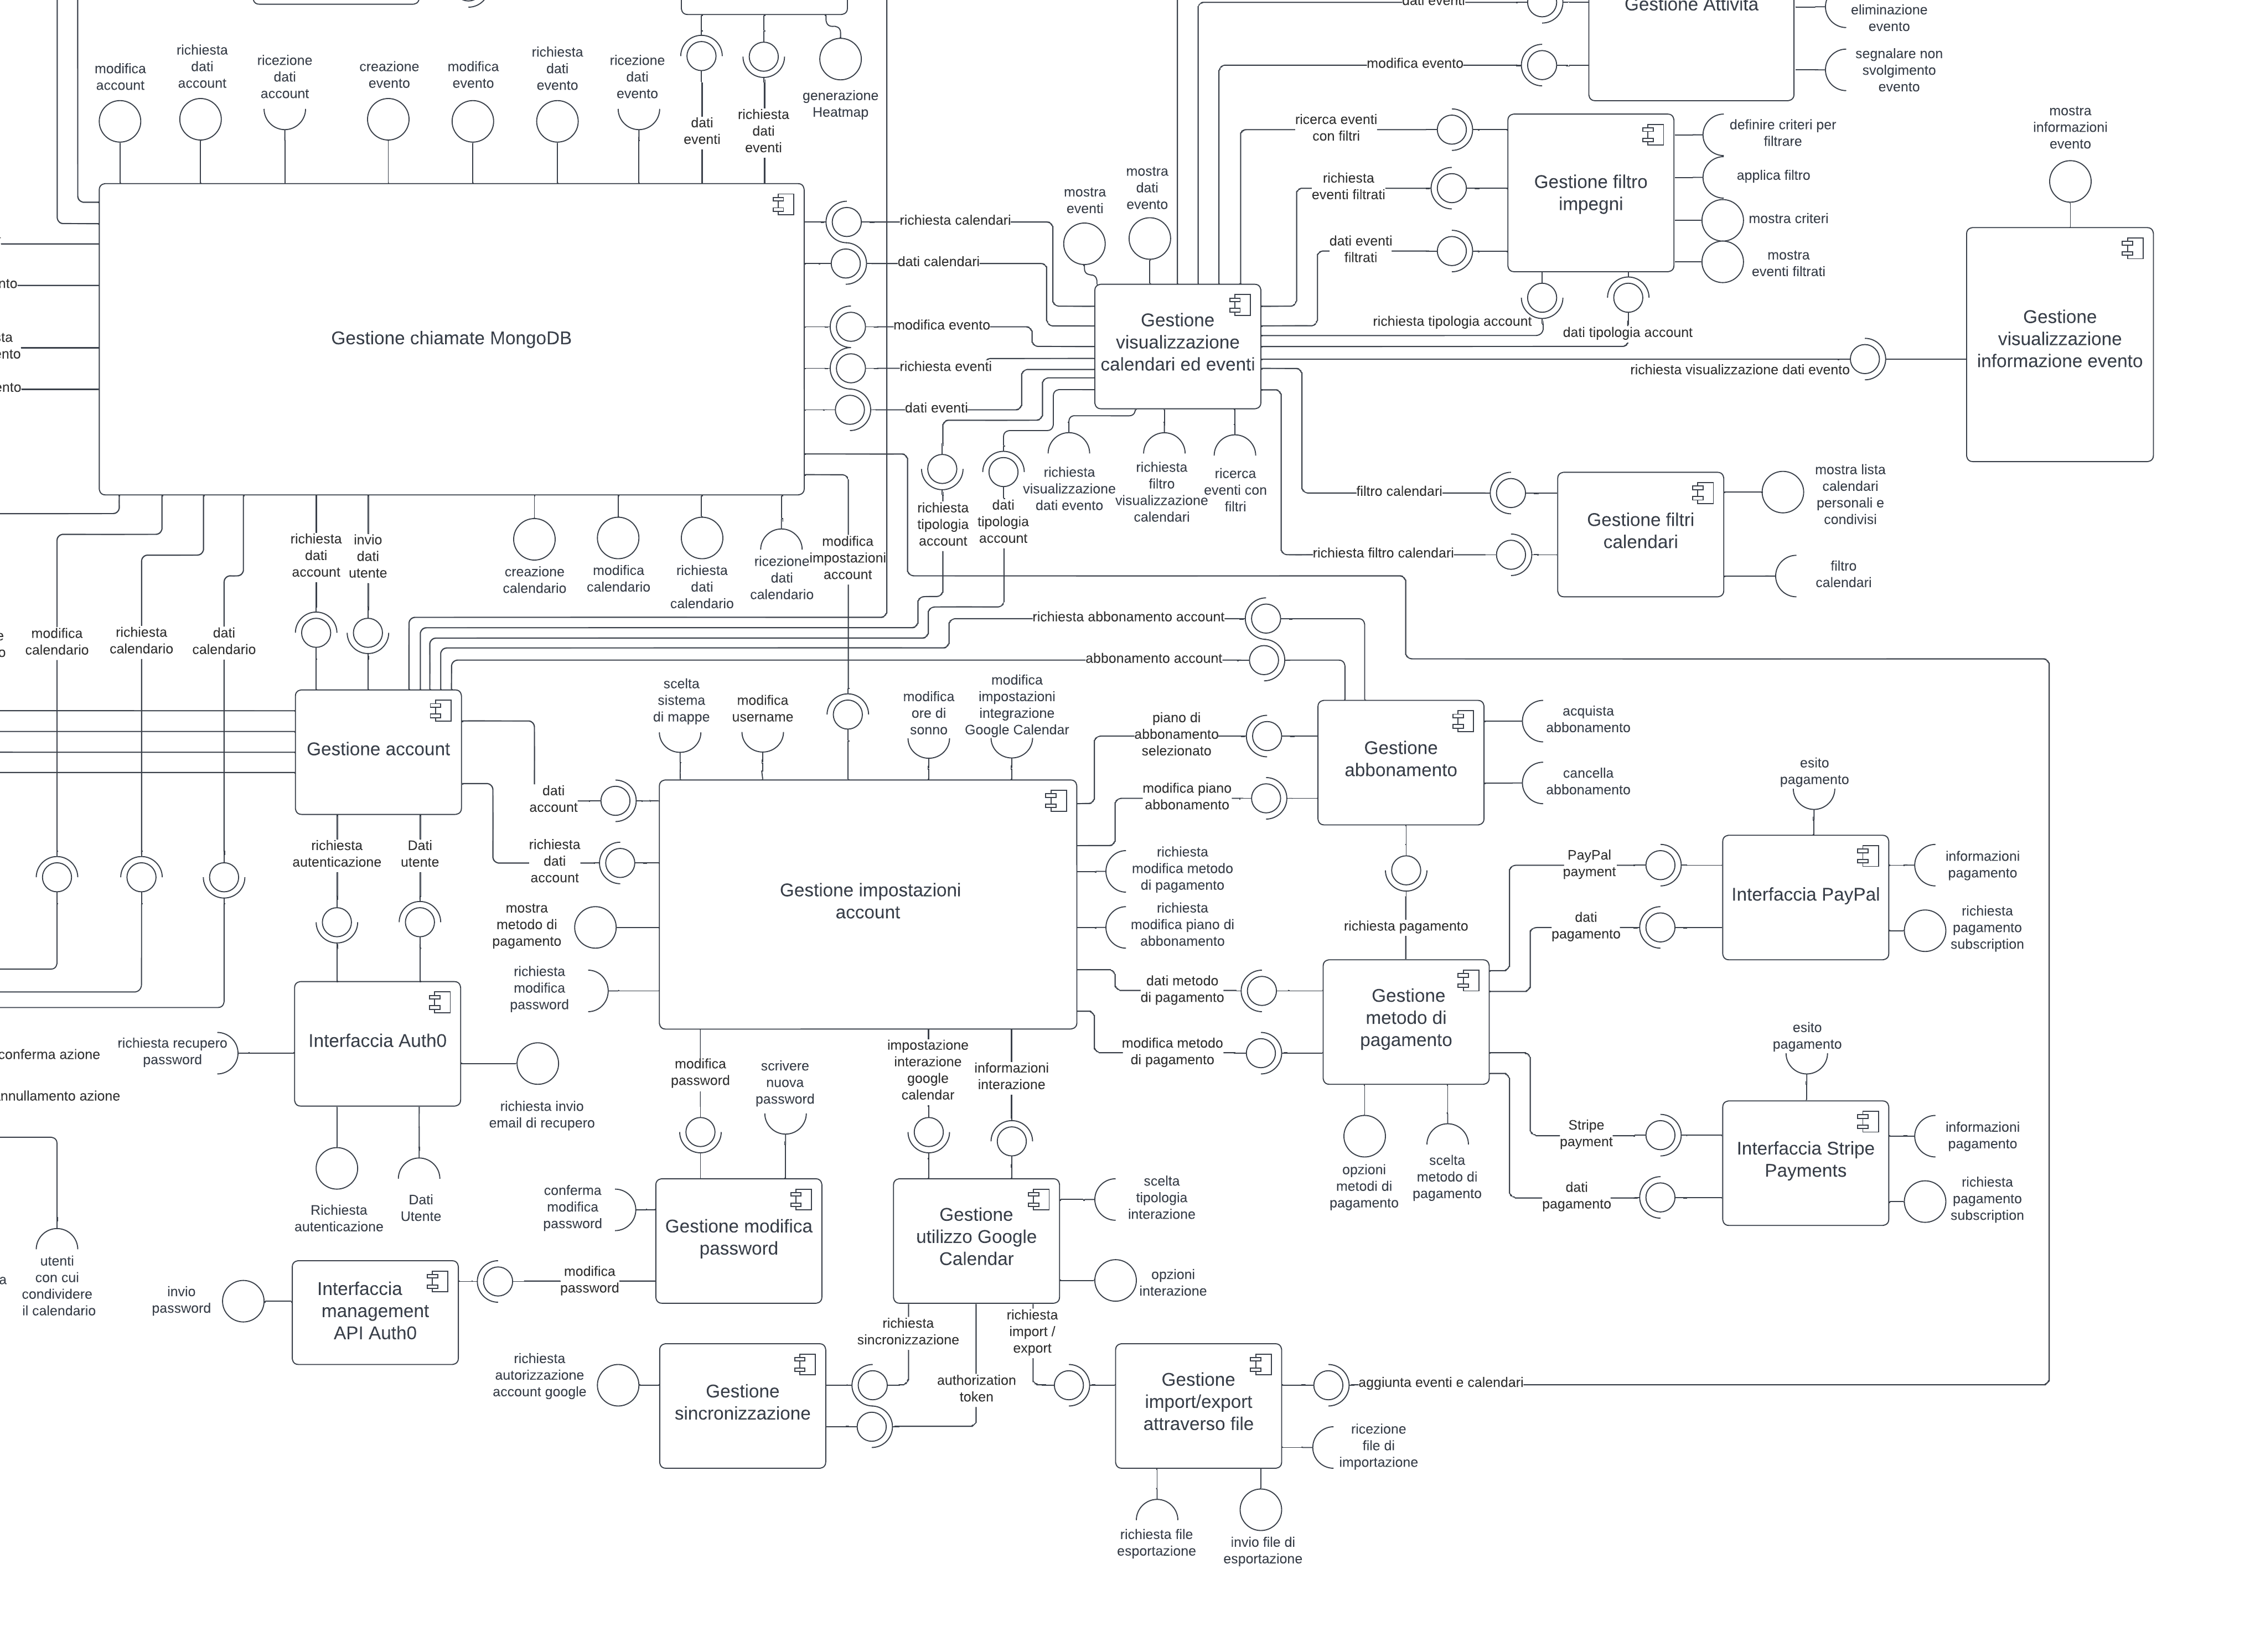
\includegraphics[width=1\textwidth,height=0.4\textheight]{img/Diagrammi/Componenti/P3_Diagramma_dei_componenti.png}
    Questa figura mostra tutto il quarto in basso a destra del diagramma dei componenti del sito PlanIt.
\end{center}
\begin{center}
    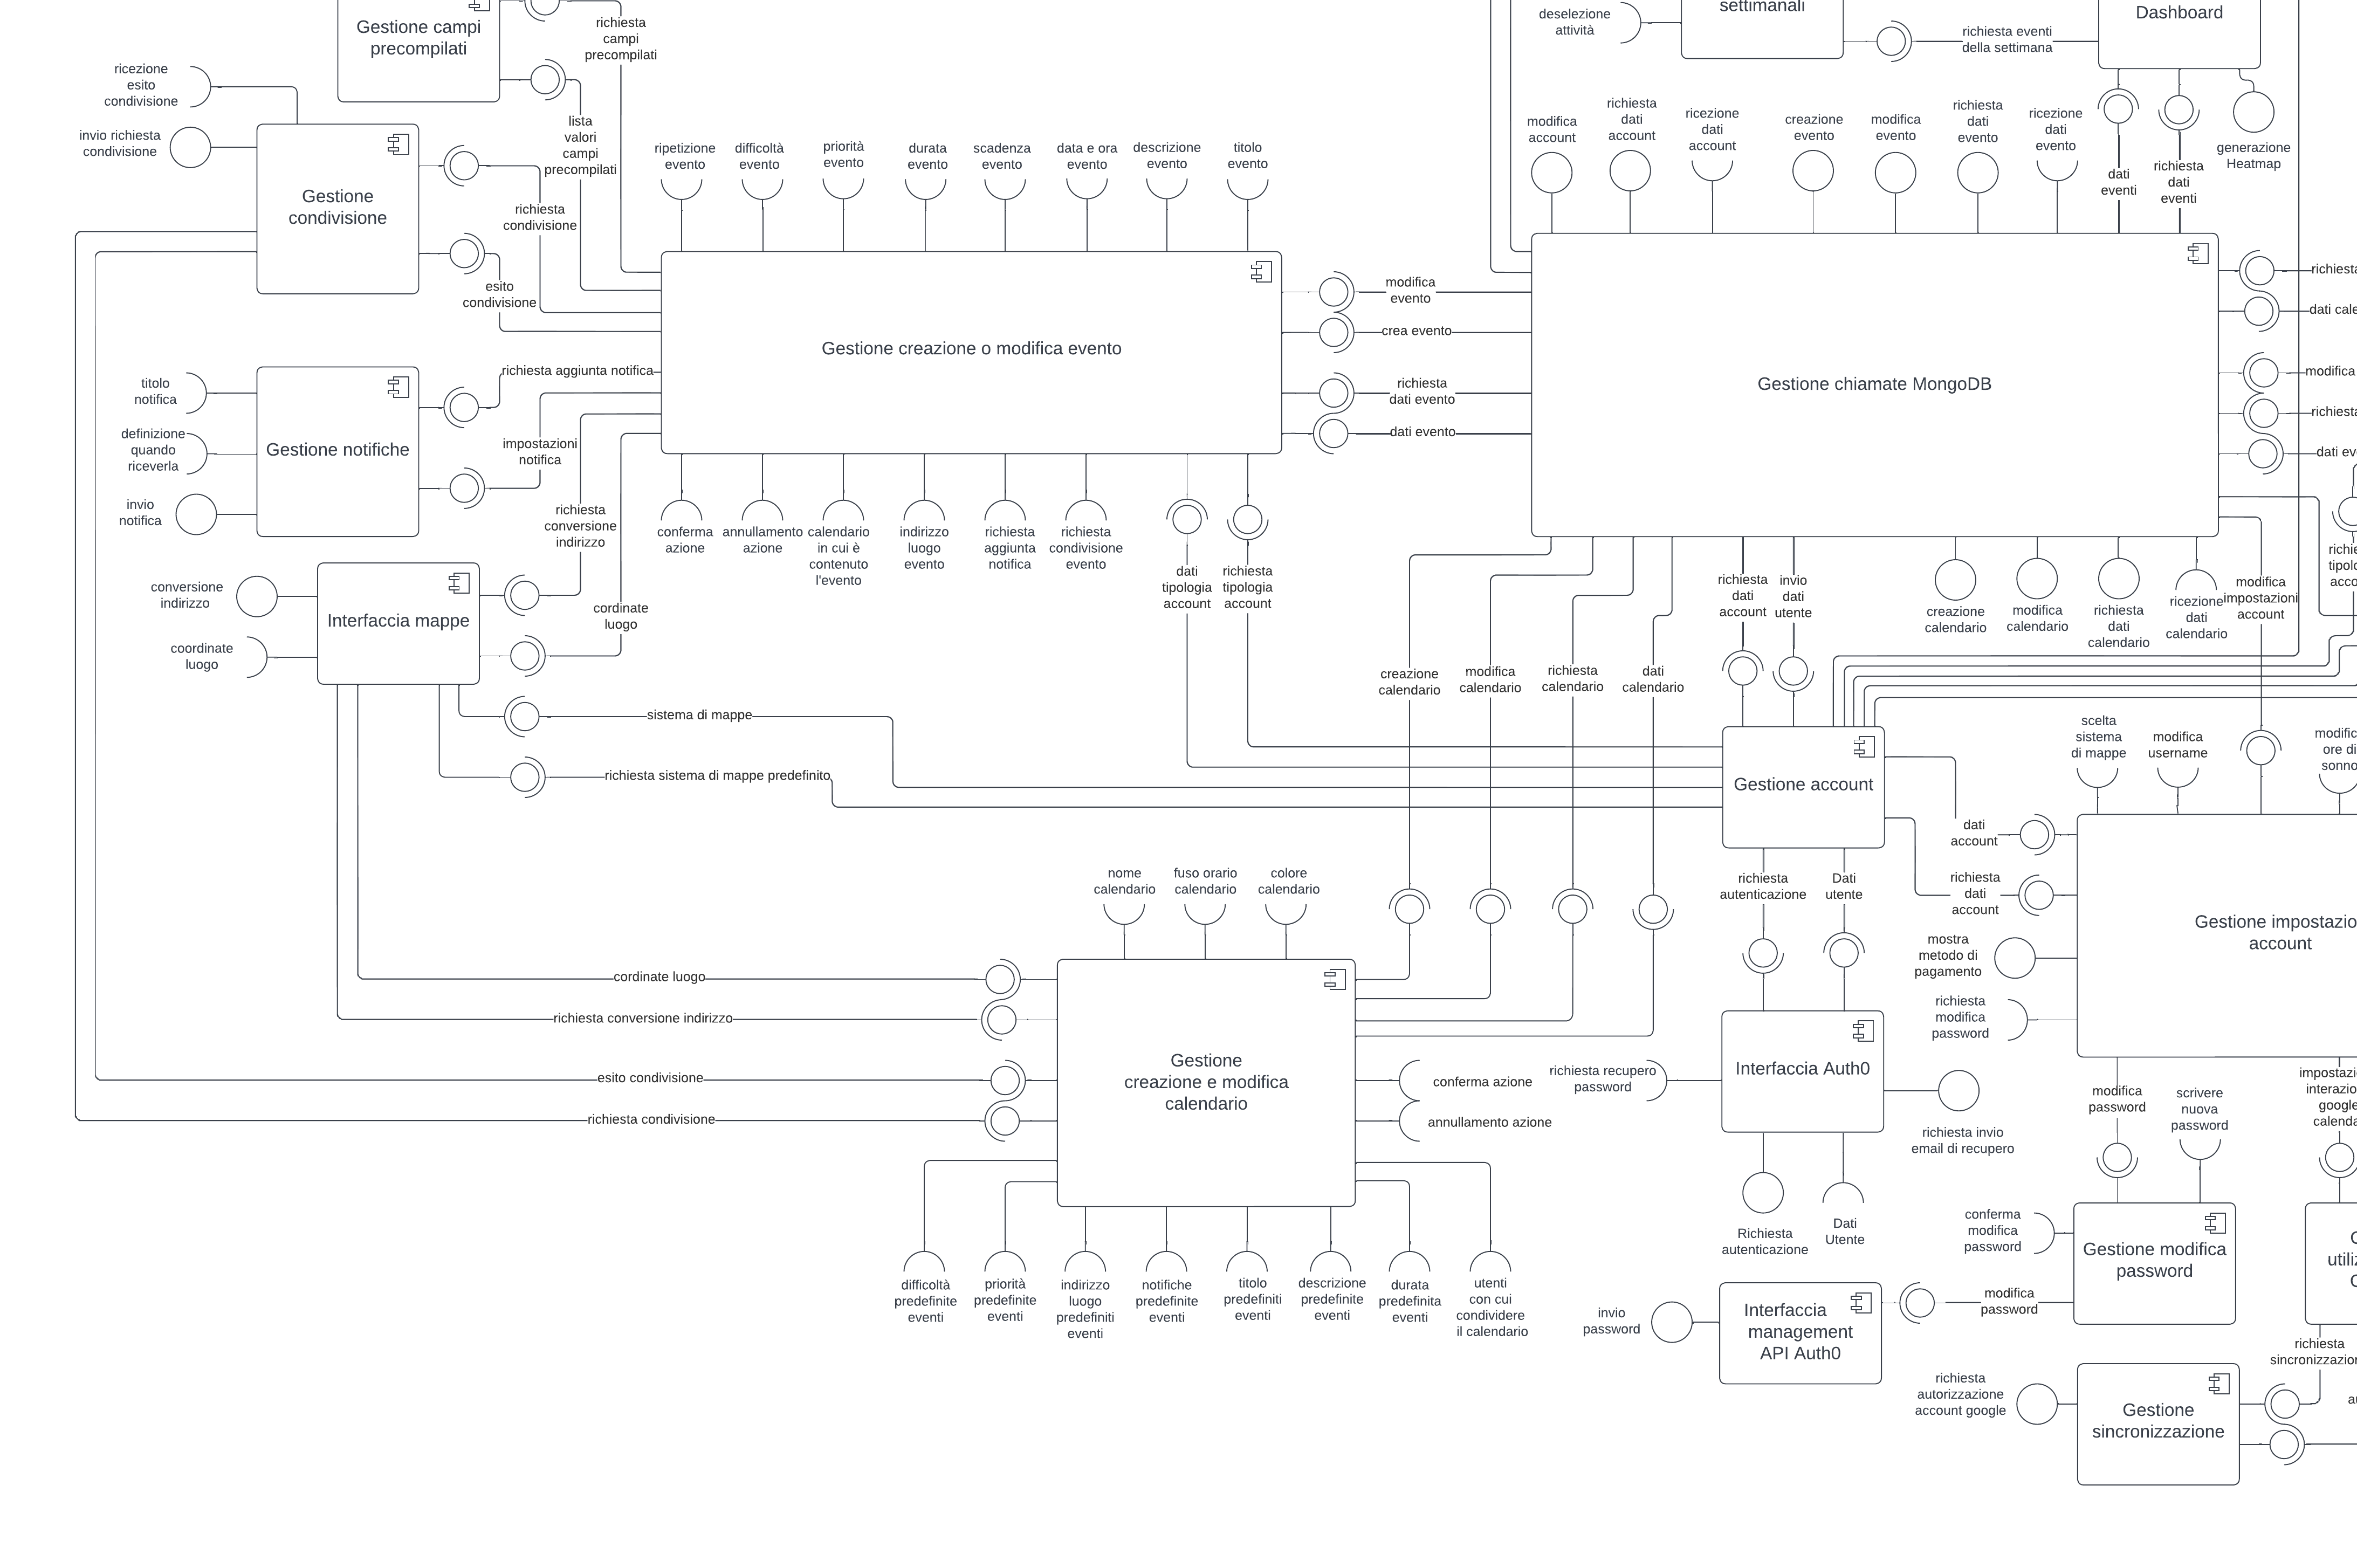
\includegraphics[width=1\textwidth,height=0.4\textheight]{img/Diagrammi/Componenti/P4_Diagramma_dei_componenti.png}
    Questa figura mostra tutto il quarto in basso a sinistra del diagramma dei componenti del sito PlanIt.
\end{center}
\newpage
\begin{listaPersonale}[DCI]{}
    \elemento[Gestione creazione o modifica evento]{dci:GestioneCreazioneModificaEvento}

    \textbf{Descrizione:} gestisce l'intera procedura che l'utente autenticato segue per creare o modificare un evento. Dopo che l'utente ha definito i campi, questo componente crea o modifica l'evento secondo i campi definiti.  Il componente fornisce una pagina dove l'utente autenticato può definire questi campi.

    \textbf{Interfaccia richiesta - ripetizione evento:} Per ripetizione evento si intende indicare quante volte l'evento, che si sta definendo, si ripete. Ricordiamo che un evento ripetuto si chiama “Abitudine”. Questo campo può anche non essere definito in tempo di creazione o modifica evento.

    \textbf{Interfaccia richiesta - difficoltà evento:} La modifica o creazione evento include la definizione, da parte dell'utente non autenticato, della difficoltà dell'evento, ovvero quanto è complesso l'evento da svolgere. Questo campo può anche non essere definito in tempo di creazione o modifica evento.

    \textbf{Interfaccia richiesta - priorità evento:} La modifica o creazione evento include la definizione, da parte dell'utente non autenticato, della priorità dell'evento, ovvero quanto è importante l'evento. Questo campo può anche non essere definito in tempo di creazione o modifica evento.

    \textbf{Interfaccia richiesta - durata evento:} L'utente non autenticato può indicare la durata dell'evento.

    \textbf{Interfaccia richiesta - deadline:} L'utente non autenticato può indicare la deadline, ovvero la scadenza, dell'evento da fare.

    \textbf{Interfaccia richiesta - data e ora evento:} L'utente non autenticato può indicare la data e ora dell'evento.

    \textbf{Interfaccia richiesta - descrizione evento:} L'utente non autenticato può definire una descrizione dell'evento, in cui scrive in modo più dettagliato cosa si farà in tale attività.

    \textbf{Interfaccia richiesta - titolo evento:} L'utente non autenticato deve definire, ogni volta che crea un evento, il titolo dell'evento.

    \textbf{Interfaccia richiesta - calendario in cui è contenuto l'evento:} L'utente autenticato (ricordiamo che l'utente non autenticato ha solo il calendario principale, quindi non può definire questo campo) può definire a quale calendario aggiungere l'evento che sta modificando o creando.

    \textbf{Interfaccia richiesta - indirizzo luogo evento:} L'utente autenticato (ricordiamo che l'utente non ha questa funzionalità) può definire il luogo dove si tiene l'evento.

    \textbf{Interfaccia fornita - richiesta conversione indirizzo:} Una volta che l'utente definisce il luogo dove si tiene l'evento, “Gestione creazione o modifica evento” richiede a “Interfaccia mappe” la conversione dell'indirizzo inserito dall'utente in coordinate luogo.

    \textbf{Interfaccia richiesta - coordinate luogo:} Dopo aver richiesto la conversione dell'indirizzo, “Gestione creazione o modifica evento” riceve le coordinate del luogo dove si terrà l'evento.

    \textbf{Interfaccia richiesta - richiesta aggiunta notifica:} L'utente autenticato (ricordiamo che l'utente non ha questa funzionalità)  può richiedere l'aggiunta della notifica per l'evento che sta creando o modificando.

    \textbf{Interfaccia fornita - richiesta aggiunta notifica:} Una volta che l'utente richiede l'aggiunta della notifica, il componente “Gestione creazione o modifica evento” manda una richiesta di aggiunta notifica al componente “Gestione notifiche”.

    \textbf{Interfaccia richiesta - impostazioni notifiche:} Dopo la richiesta aggiunta notifica, “Gestione creazione o modifica evento” riceve le impostazioni notifica definite.

    \textbf{Interfaccia richiesta - richiesta condivisione:} L'utente (ricordiamo che l'utente non ha questa funzionalità) può richiedere la condivisione dell'evento con altri utenti autenticati.

    \textbf{Interfaccia fornita - richiesta condivisione:} Dopo che l'utente ha richiesto la condivisione dell'evento, il componente “Gestione creazione o modifica evento” richiede la condivisione dell'evento al componente “Gestione condivisione”

    \textbf{Interfaccia richiesta - esito condivisione:} Dopo che la condivisione è stata processata, “Gestione creazione o modifica evento” riceve l'esito della condivisione, che può esser stata accettata o meno dall'utente a cui abbiamo inviato la condivisione.

    \textbf{Interfaccia richiesta - conferma azione:} L'utente non autenticato, quando reputa di aver finito la creazione o modifica evento, segnala la conferma dell'azione compiuta.

    \textbf{Interfaccia richiesta - annullamento azione:} L'utente non autenticato può anche abortire la creazione o modifica evento, annullando l'azione.

    \textbf{Interfaccia richiesta - lista valori precompilati:} Quando l'utente definisce il calendario in cui aggiungere l'evento interessato, il componente “Gestione creazione o modifica evento” richiede a “Gestione campi precompilati” i campi precompilati del calendario in cui aggiungiamo l'evento. I campi precompilati sono definiti nelle “Impostazioni predefinite di un calendario”.
    I campi precompilati riguardano:
    \begin{itemize}
        \item priorità;
        \item difficoltà;
        \item impostazioni notifiche;
        \item descrizione e titolo;
        \item luogo evento;
    \end{itemize}

    \textbf{Interfaccia fornita - lista valori precompilati:}  Dopo la richiesta dei valori precompilati, “Gestione creazione o modifica evento” riceve la lista dei valori precompilati.

    \textbf{Interfaccia fornita - richiesta dati evento:} Quando l'utente chiede la modifica di un evento, “Gestione creazione o modifica evento” richiede i dati dall'evento da modificare a "Gestione chiamate MongoDB”

    \textbf{Interfaccia fornita - modifica evento:} Nel caso della modifica di un evento preesistente, il componente invierà le modifiche evento a “Gestione chiamate MongoDB”.

    \textbf{Interfaccia fornita - crea evento:} Nel caso della creazione di un nuovo evento, “Gestione creazione o modifica evento” invia l'evento creato a “Gestione chiamate MongoDB”.

    \textbf{Interfaccia fornita - richiesta tipologia account:} Il componente “Gestione creazione o modifica evento” richiede a “Gestione account”  la tipologia account dell'utente che sta andando a creare o modificare l'evento. In questo modo il componente può sapere quali campi rendere disponibili alla modifica o creazione all'utente interessato. Infatti un utente non autenticato non può definire i seguenti campi, in quanto riguardano funzionalità non presenti nel suo piano account:
    \begin{itemize}
        \item luogo evento;
        \item notifica;
        \item lista degli utenti a cui è condiviso il calendario;
    \end{itemize}

    \textbf{Interfaccia richiesta - dati tipologia account:} Il componente “Gestione creazione o modifica evento” riceve i dati tipologia account, per poter presentare all'utente interessato i campi di creazione o modifica a lui disponibili.


    \elemento[Gestione notifiche]{dci:GestioneNotifiche}

    \textbf{Descrizione:} gestione notifiche gestisce la funzionalità di creazione o modifica della notifica di un evento, dopo che l'utente ha definito dei campi d'impostazione della notifica.

    \textbf{Interfaccia richiesta - titolo notifica:} “Gestione notifiche” può ricevere dall'utente autenticato standard il titolo della notifica da creare.

    \textbf{Interfaccia richiesta - definizione quando riceverla:} “Gestione notifiche” può ricevere dall'utente autenticato standard quanto prima rispetto all'evento deve inviare la notifica.

    \textbf{Interfaccia fornita - invio notifica:} Il componente “Gestione notifiche”, una volta creato la notifica con le impostazioni date dall'utente autenticato standard, gestisce anche l'invio della notifica all'evento secondo le impostazioni poste dall'utente autenticato standard.

    \textbf{Interfaccia richiesta - richiesta aggiunta notifica:} “Gestione notifiche” ha bisogno della richiesta “aggiunta notifica” per iniziare la procedura di creazione della notifica.

    \textbf{Interfaccia fornita - impostazioni notifica:} Il componente, dopo la creazione della notifica, fornisce le impostazioni notifica al componente “Gestione creazione o modifica evento”, in modo tale che anche l'evento creato possa avere le impostazioni della notifica creata.


    \elemento[Interfaccia sistema di mappe]{dci:InterfacciaMappe}

    \textbf{Descrizione:} il componente gestisce la funzionalità data all'utente standard di interagire con un sistema esterno di mappe per definire il luogo dove avviene l'evento, gestendo l'intera procedura, ovvero invio del luogo al sistema esterno di mappe e ricezione delle coordinate di questo.

    \textbf{Interfaccia richiesta - richiesta conversione indirizzo:}   Il componente “Interfaccia mappe” inizia la procedura di ottenimento delle coordinate di un luogo, solo una volta ottenuto l'indirizzo del luogo da “Gestione creazione o modifica evento” o da “Gestione creazione e modifica calendario”.

    \textbf{Interfaccia fornita - conversione indirizzo:} Per ottenere le coordinate dell'indirizzo inserito dall'utente, il componente “Interfaccia sistema di mappe” deve inviare questo indirizzo al sistema di mappe esterno. Il sistema di mappe esterno utilizzato è o OpenStreetMap o Google Maps: la scelta di uno dei due viene fatto dall'utente autenticato standard in impostazioni account.

    \textbf{Interfaccia richiesta - coordinate luogo:} Dopo aver inviato l'indirizzo, il componente “Interfaccia mappe” ottiene le coordinate luogo dal sistema di mappe esterno.

    \textbf{Interfaccia fornita - coordinate luogo:} Il componente “Interfaccia mappe”, ottenendo le coordinate luogo dal sistema mappe esterno, invia l'indirizzo del luogo a “Gestione creazione o modifica evento” o a “Gestione creazione e modifica calendario”, in modo tale che l'evento e calendario creato o modificato abbia anche le coordinate del luogo dove si terrà l'evento.


    \elemento[Gestione condivisione]{dci:GestioneCondivisione}


    \textbf{Descrizione:} il componente “Gestione condivisione” gestisce la condivisione di eventi e calendari, ovvero fa in modo di creare la condivisione di eventi e calendari tra utenti sovrintendono l'intera procedura di condivisione fino alla ricevuta dell'esito di condivisione.

    \textbf{Interfaccia richiesta - richiesta condivisione:} Il componente “Gestione condivisione” inizia la procedura di condivisione solo una volta ottenuta la richiesta condivisione da “Gestione creazione o modifica evento” o da “Gestione creazione e modifica calendario”. La richiesta di condivisione contiene anche l'username degli utenti autenticato standard con cui si vuole condividere l'evento.

    \textbf{Interfaccia fornita - invio richiesta condivisione:} Il componente “Gestione condivisione” invia la richiesta di condivisione all'utente autenticato standard ottenuto nella richiesta condivisione.

    \textbf{Interfaccia richiesta - ricezione esito condivisione:} Il componente “Gestione condivisione”, una volta che l'utente autenticato standard ricevente della condivisione accetta o rifiuta la condivisione dell'evento, ottiene la sua risposta e quindi l'esito della condivisione.

    \textbf{Interfaccia fornita - esito condivisione:} Il componente “Gestione condivisione” invia l'esito della condivisione a “Gestione creazione o modifica evento” o a “Gestione creazione e modifica calendario” in modo tale che l'evento o il calendario creato possa contenere l'informazione sulla buona riuscita o meno della condivisione.


    \elemento[Gestione campi precompilati]{dci:GestioneCampiPrecompilati}

    \textbf{Descrizione:}  “Gestione campi precompilati” è fornire i campi precompilati di creazione o modifica evento di un specifico calendario, i quali sono definiti nelle “Impostazioni predefinite di un calendario”.

    \textbf{Interfaccia richiesta - richiesta campi precompilati:} Il componente “Gestione campi precompilati” per iniziare la procedura di ottenimento e invio dei campi precompilati di un evento appartenente ad un calendario, deve ricevere una richiesta da “Gestione creazione o modifica calendario” contenente anche il calendario in cui va inserito l'evento che sta creando o modificando “Gestione creazione o modifica evento”.

    \textbf{Interfaccia fornita - richiesta dati calendario:} Il componente “Gestione campi precompilati” per ottenere i campi precompilati di un evento appartenente di un calendario deve richiedere alla “Gestione chiamate MongoDB” i dati del calendario, nello specifico le impostazioni predefinite del calendario, dove è presente:
    \begin{itemize}
        \item priorità;
        \item difficoltà;
        \item impostazioni notifiche;
        \item descrizione e titolo;
        \item luogo evento;
    \end{itemize}

    \textbf{Interfaccia richiesta - dati calendario:} Dopo aver mandato la richiesta di dati calendario, il componente “Gestione campi precompilati” ottiene i dati del calendario, nello specifico i dati indicati in “interfaccia fornita - richiesta dati calendario”.

    \textbf{Interfaccia fornita - lista valori campi precompilati:} Dopo aver ottenuto i dati calendario, il componente “Gestione campi precompilati” invia a “Gestione creazione o modifica calendario” la lista con i valori dei campi precompilati usati nella creazione o modifica di un evento appartenente ad un calendario.


    \elemento[Gestione creazione e modifica calendario]{dci:GestioneCreazioneModificaCalendario}

    \textbf{Descrizione:} il componente gestisce la creazione e modifica di calendari da parte dell'utente autenticato standard. Nello specifico, questo componente gestisce l'intera procedura di questa funzionalità, creando o modificando un calendario secondo dei campi definiti dall'utente non autenticato.

    \textbf{Interfaccia richiesta - nome calendario:} Il componente “Gestione creazione o modifica calendario” ottiene dall'utente non autenticato il nome del calendario in fase di creazione e modifica calendario.

    \textbf{Interfaccia richiesta - fuso orario:} Il componente può ottenere dall'utente non autenticato il fuso orario del calendario.

    \textbf{Interfaccia richiesta - colore:} Il componente “Gestione creazione o modifica calendario”, in fase di creazione o modifica di un calendario, può ottenere dall'utente non autenticato il colore del calendario, ovvero il colore con cui sono sono mostrati gli eventi all'interno della pagina “Calendario” (vedi \prettyref{D1-fe:SchermataPrincipale})

    \textbf{Interfaccia richiesta - utenti con cui condividere il calendario:} Il componente “Gestione creazione o modifica calendario” può ottenere da un utente autenticato standard gli utenti a cui il calendario è condiviso. Questa interfaccia non è disponibile, ricordiamo, agli utenti non autenticati

    \textbf{Interfaccia richiesta - priorità predefinite eventi:} Il componente “Gestione creazione o modifica calendario” può ottenere dall'utente non autenticato standard la priorità con cui tutte le priorità degli eventi appartenenti a questo calendario saranno precompilate. Ovviamente, in fase di creazione o modifica evento, questa priorità precompilata può essere modificata.

    \textbf{Interfaccia richiesta - indirizzo luogo predefiniti eventi:} Il componente “Gestione creazione o modifica calendario” può ottenere dall'utente autenticato standard l'indirizzo con cui tutti i campi luoghi degli eventi appartenenti a questo calendario saranno precompilati. Ovviamente, in fase di creazione o modifica evento, l'indirizzo precompilata può essere modificato. Questa interfaccia non è disponibile, ricordiamo, agli utenti non autenticati.

    \textbf{Interfaccia richiesta - difficoltà predefinite eventi:} Il componente “Gestione creazione o modifica calendario” può ottenere dall'utente non autenticato la difficoltà con cui tutte le difficoltà degli eventi appartenenti a questo calendario saranno precompilate. Ovviamente, in fase di creazione o modifica evento, questa difficoltà precompilata può essere modificata.

    \textbf{Interfaccia richiesta - notifiche predefinite eventi:} Il componente “Gestione creazione o modifica calendario” può ottenere dall'utente autenticato standard le impostazioni della notifica con cui tutte le notifiche degli eventi appartenenti a questo calendario saranno definite. Ovviamente, in fase di creazione o modifica evento, le impostazioni della notifica dell'evento precompilate possono essere modificate. Questa interfaccia non è disponibile, ricordiamo, agli utenti non autenticati.

    \textbf{Interfaccia richiesta - titolo predefiniti eventi:} Il componente “Gestione creazione o modifica calendario” può ottenere dall'utente non autenticato il titolo con cui tutti i titoli degli eventi appartenenti a questo calendario saranno precompilati. Ovviamente, in fase di creazione o modifica evento, il titolo precompilata può essere modificato.

    \textbf{Interfaccia richiesta - descrizioni predefinite eventi:} Il componente “Gestione creazione o modifica calendario” può ottenere dall'utente non autenticato la descrizione con cui tutte le descrizioni degli eventi appartenenti a questo calendario saranno precompilate. Ovviamente, in fase di creazione o modifica evento, la descrizione precompilata può essere modificata.

    \textbf{Interfaccia richiesta - durata predefinita eventi:} Il componente “Gestione creazione o modifica calendario” può ottenere dall'utente non autenticato la durata con cui tutte le durate degli eventi appartenenti a questo calendario saranno precompilate. Ovviamente, in fase di creazione o modifica evento, la durata precompilata può essere modificata.

    \textbf{Interfaccia richiesta - conferma azione:} Il componente, una volta che l'utente non autenticato ha finito l'azione di creazione o modifica calendario,  deve ottenere la conferma azione, in modo da salvare le modifiche fatte.

    \textbf{Interfaccia richiesta - annullamento azione:} Il componente potrebbe ricevere dall'utente non autenticato l'annullamento dell'azione, causando l'aborto di tutte le azioni fatte dall'utente non autenticato e il non salvataggio delle modifiche fatte.

    \textbf{Interfaccia fornita - richiesta conversione indirizzo:} Una volta che l'utente definisce il luogo dove si tengono gli eventi del calendario che si sta o creando o modificando, “Gestione creazione o modifica calendario” richiede a “Interfaccia mappe” la conversione dell'indirizzo inserito dall'utente in coordinate luogo.

    \textbf{Interfaccia richiesta - coordinate luogo:} Dopo aver richiesto la conversione dell'indirizzo, “Gestione creazione o modifica calendario” riceve le coordinate del luogo dove si terranno di default gli eventi.

    \textbf{Interfaccia fornita - richiesta condivisione:} Dopo che l'utente ha richiesto la condivisione dell'evento, il componente “Gestione creazione o modifica calendario” richiede la condivisione dell'evento al componente “Gestione condivisione”.

    \textbf{Interfaccia richiesta - esito condivisione:} Dopo che la condivisione è stata processata, “Gestione creazione o modifica calendario” riceve l'esito della condivisione, che può esser stata accettata o meno dall'utente a cui abbiamo inviato la condivisione.


    \elemento[Gestione Dashboard]{dci:GestioneDashBoard}

    \textbf{Descrizione:} il componente “Dashboard” permette all'utente autenticato di ottenere delle informazioni sull'uso del tempo,  mostrando dati sulle attività dell'utente non autenticato in base ad alcuni periodi di tempo.

    \textbf{Interfaccia fornita - heatmap:}  “Gestione Dashboard” mostra una heatmap il cui scopo è rappresentare il tempo che deve essere dedicato ogni giorno per rispettare le varie scadenze, considerando un periodo di tempo fino al semestre.

    \textbf{Interfaccia fornita - richiesta dati eventi:} “Gestione Dashboard” richiede a “Gestione chiamate MongoDB” i dati eventi, ovvero gli eventi con le loro rispettive informazioni che non sono altro che i campi definiti durante la creazione o modifica evento.

    \textbf{Interfaccia richiesta - dati eventi:} Una volta che “Gestione Dashboard” invia la richiesta di dati eventi, ottiene da “Gestione chiamate MongoDB” i dati eventi.

    \textbf{Interfaccia richiesta - richiesta eventi giornalieri:} “Gestione Dashboard” riceve la richiesta di eventi giornalieri, ovvero la lista degli eventi della giornata con le loro rispettive informazioni.
    Gli eventi giornalieri sono ottenuti da questo componente filtrando i dati eventi prendendo solo quelli della giornata attuale.

    \textbf{Interfaccia fornita - dati eventi giornalieri:} “Gestione Dashboard” fornisce “Gestione eventi giornalieri” i dati degli eventi giornalieri, ovvero gli eventi giornalieri con le loro rispettive informazioni. I dati eventi giornalieri vengono filtrati dai dati eventi, presi, come descritto precedentemente, da “Gestione chiamate MongoDB”.

    \textbf{Interfaccia richiesta - richiesta eventi della settimana:} “Gestione Dashboard” riceve la richiesta di eventi della settimana, ovvero la lista degli eventi della giornata con le loro rispettive informazioni. Gli eventi settimanali sono ottenuti da questo componente filtrando i dati eventi prendendo solo quelli della settimana attuale.

    \textbf{Interfaccia fornita - dati eventi della settimana:} “Gestione Dashboard” fornisce  “Gestione eventi settimanali” i dati degli eventi settimanali, ovvero gli eventi settimanali con le loro rispettive informazioni. I dati eventi settimanali vengono filtrati dai dati eventi, presi, come descritto precedentemente, da “Gestione chiamate MongoDB”.


    \elemento[Gestione eventi settimanali]{dci:GestioneEventiSettimanali}

    \textbf{Descrizione:} il componente “Gestione attività settimanali” fa in modo di fornire delle informazioni sulle attività settimanali all'utente non autenticato mostrando un grafico a barre.

    \textbf{Interfaccia fornita - richiesta eventi della settimana:} “Gestione attività settimanali”, per fornire le proprie funzionalità, deve avere i dati eventi della settimana, i quali richiede a “Gestione Dashboard”.

    \textbf{Interfaccia richiesta - dati eventi della settimana:} “Gestione attività settimanali”, dopo aver fatto la richiesta degli eventi della settimana, ottiene da “Gestione Dashboard” i dati eventi della settimana.

    \textbf{Interfaccia fornita - generazione grafico a barre:} Il componente, una volta ottenuto gli eventi della settimana con le loro rispettive informazioni, genera e mostra un grafico a barre visualizzabile dall'utente non autenticato. Questo grafico a barre generato può anche avere evidenziata un'attività selezionata dall'utente non autenticato.

    \textbf{Interfaccia richiesta - selezione attività:} Il componente “Gestione attività settimanali” può ricevere la selezione di un'attività dalla legenda del grafico, generando un grafico a barre delle attività della settimana con tale evento evidenziato.

    \textbf{Interfaccia richiesta - deselezione attività:} Il componente, una volta che ha ricevuto la selezione di un'attività, può ricevere anche la deselezione di quest'ultimo, facendo tornare il grafico a barre al suo stato originale con nessuna attività evidenziata.


    \elemento[Gestione eventi giornalieri]{dci:GestioneEventiGiornalieri}

    \textbf{Descrizione:} il componente “Gestione attività giornaliere” mostra un grafico a torta e una lista delle attività giornaliere, gestisce la sincronizzazione tra i due grafici e l'interazione dell'utente non autenticato con la lista delle attività giornaliere.

    \textbf{Interfaccia fornita - mostra grafico a torta:} Il componente “Gestione eventi giornalieri” mostra un grafico a torta contenente le attività presenti nella lista di attività giornaliere. Gli eventi nel grafico a torta presentano una dimensione proporzionata alla loro durata.

    \textbf{Interfaccia fornita - mostra lista calendari o eventi:} Il componente “Gestione eventi giornalieri” mostra la lista delle attività giornaliere con a fianco la loro durata. Questa lista può subire delle interazioni con l'utente non autenticato, portando alla modifica di questa.

    \textbf{Interfaccia richiesta - esplora calendario:} Il componente potrebbe ricevere da un utente non autenticato l'esplorazione, premendo, di un calendario presente nella lista di attività (ricordiamo che un calendario può essere considerato un'attività che raggruppa sottoattività, f.e. calendario lavoro contiene le sottoattività “scrivere requisiti funzionali”, “scrivere requisiti non funzionali”, ecc..) ottenendo la visualizzazione delle sottoattività della giornata di tale calendario al posto della lista di tutte le attività giornaliere; contestualmente il grafico a torta mostrerà tutte le sottoattività del calendario, nascondendo le altre attività giornaliere.

    \textbf{Interfaccia richiesta - seleziona attività:} L'utente non autenticato, mettendo il puntatore sopra ad una delle attività della lista attività, fa in modo che il componente “Gestione eventi giornalieri” mostri evidenziata l'attività di cui si ha il cursore sopra nel grafico a torta.

    \textbf{Interfaccia fornita - richiesta eventi giornalieri:} “Gestione eventi giornalieri”, per fornire le proprie funzionalità, deve avere i dati eventi della giornata, i quali richiede a “Gestione Dashboard”.

    \textbf{Interfaccia richiesta - dati eventi giornalieri:} “Gestione eventi giornalieri”, dopo aver fatto la richiesta degli eventi della settimana, ottiene da “Gestione Dashboard” i dati eventi della giornata.


    \elemento[Gestione impostazioni account]{dci:GestioneImpostazioniAccount}

    \textbf{Descrizione:} Il componente “Gestione impostazioni account” permette all'utente autenticato di modificare e salvare le modifiche fatte ad un account di un utente autenticato standard.

    \textbf{Interfaccia richiesta - scelta sistema di mappe:} Il componente “Gestione impostazioni account” permette all'utente autenticato standard di scegliere tra Google Maps e OpenStreetMap, sistemi esterni utilizzati dal sistema per calcolare le coordinate del luogo dove si tiene l'evento, quando l'utente autenticato standard va ad indicare l'indirizzo di questo.

    \textbf{Interfaccia richiesta - modifica username:} Il componente “Gestione impostazioni account” può gestire la modifica dell'username da parte di un utente autenticato standard.

    \textbf{Interfaccia richiesta - modifica ore di sonno:} Il componente “Gestione impostazioni account” può ricevere dall'utente autenticato standard la definizione delle proprie ore di sonno. Le ore di sonno definite saranno poste in tutti i calendari posseduti dall'utente autenticato standard.
    \textbf{Interfaccia richiesta - modifica impostazioni integrazione
        Google Calendar:} Il componente “Gestione impostazioni account” può ricevere dall'utente autenticato standard la richiesta di modificare il metodo di interazione con Google Calendar. Infatti l' interazione con Google Calendar, come già citato, può essere fatta o in maniera manuale o automatica.

    \textbf{Interfaccia fornita - mostra metodo di pagamento:} Il componente mostra il metodo di pagamento scelto dall'utente autenticato premium per pagare il proprio piano di abbonamento al sito.
    \textbf{Interfaccia richiesta - richiesta modifica metodo di
        pagamento:} Il componente “Gestione impostazioni account” può ricevere dall'utente autenticato premium la richiesta di modifica del metodo di pagamento.

    \textbf{Interfaccia fornita - modifica metodo di pagamento:} Una volta che “Gestione impostazioni account” riceve la richiesta di modifica del metodo di pagamento da parte dell'utente autenticato standard, invierà la richiesta del metodo di pagamento al componente “Gestione metodo di pagamento”.

    \textbf{Interfaccia richiesta - dati metodo di pagamento:} Dopo aver richiesto la modifica del metodo di pagamento a “Gestione metodo di pagamento”, il quale gestirà la modifica del metodo di pagamento, il componente “Gestione impostazioni account” riceve i dati del metodo di pagamento selezionato.

    \textbf{Interfaccia richiesta - richiesta modifica password:} Il componente“Gestione impostazioni account” può ricevere dall'utente autenticato standard la richiesta di modifica password.

    \textbf{Interfaccia richiesta - modifica password:} Il componente, in seguito aver ricevuto la richiesta di modifica password da parte dell'utente autenticato standard, invierà la richiesta al componente “Gestione modifica password” che gestirà la modifica della password.

    \textbf{Interfaccia fornita - modifica impostazioni account:} Una volta che l'utente autenticato standard avrà modificato e salvato le modifiche alle impostazioni del proprio account, questo componente invierà a “Gestione chiamate MongoDB” la modifica delle impostazioni account dell'utente autenticato standard interessato.
    \textbf{Interfaccia richiesta - richiesta modifica piano di
        abbonamento:} Il componente “Gestione impostazioni account” può ricevere dall'utente autenticato standard la richiesta di modifica del metodo di abbonamento, ovvero il passaggio da utente autenticato standard a premium o viceversa.

    \textbf{Interfaccia fornita - modifica piano di abbonamento:} Una volta che “Gestione impostazioni account” riceve la richiesta di modifica del piano di abbonamento da parte o dell'utente autenticato standard o premium, invierà la richiesta di modifica piano di abbonamento al componente “Gestione abbonamento”.

    \textbf{Interfaccia richiesta - piano di abbonamento selezionato:} Dopo aver richiesto la modifica del piano di abbonamento a “Gestione abbonamento”, il quale gestirà la modifica del piano di abbonamento, il componente riceve il piano di abbonamento selezionato.
    \textbf{Interfaccia fornita - impostazioni integrazione Google
        Calendar:} Dopo aver ricevuto dall'utente autenticato standard la richiesta di modifica delle impostazioni di integrazione con Google Calendar, il componente “Gestione impostazioni account” invia la richiesta di modifica a “Gestione utilizzo Google Calendar”.

    \textbf{Interfaccia richiesta - informazioni integrazione:} Dopo aver richiesto la modifica delle impostazioni di integrazione con Google Calendar a “Gestione utilizzo Google Calendar”, il quale gestirà la modifica di queste impostazioni, il componente “Gestione impostazioni account” riceve informazioni riguardo l'integrazione, ovvero la scelta del metodo di integrazione con Google Calendar.

    \textbf{Interfaccia fornita - richiesta dati account:} Il componente richiede al componente “Gestione account” i dati account dell'utente autenticato standard.

    \textbf{Interfaccia richiesta - dati account:} Il componente, dopo aver richiesto i dati account, riceve, da “Gestione account” i dati account, ovvero tipologia di abbonamento, sistema di mappe predefinito, username, sistema di pagamento predefinito, informazioni riguardanti al pagamento tramite paypal, informazioni riguardanti al pagamento tramite stripe, numero di ore sonno e le impostazioni della integrazione con Google calendar. Tutti questi dati account servono al componente “Gestione impostazioni account” per mostrare all'utente autenticato standard le impostazioni del proprio account.


    \elemento[Gestione modifica password]{dci:GestioneModificaPassword}

    \textbf{Descrizione:} il componente “Gestione modifica password” implementa la funzionalità modifica della password per un utente autenticato standard.

    \textbf{Interfaccia richiesta - modifica password:} Il componente “Gestione modifica password” riceve la richiesta di modifica password da “Gestione impostazioni account”,

    \textbf{Interfaccia richiesta - scrivere nuova password:} Il componente riceve dall'utente autenticato standard la nuova password.

    \textbf{Interfaccia richiesta - conferma modifica password:} Il componente riceve dall'utente la conferma dell'operazione di modifica password

    \textbf{Interfaccia fornita - modifica la password:} Dopo aver ricevuto la nuova password, il componente “Gestione modifica password” invia la nuova password a “Interfaccia management API Auth0”.


    \elemento[Interfaccia API Auth0]{dci:InterfacciaAPIAuth0}

    \textbf{Descrizione:} il componente, dopo aver valutato che la nuova password rispetti i criteri minimi di sicurezza, aggiorna la password nel database credenziali presente in Auth0 tramite le rest API di Auth0 management.

    \textbf{Interfaccia richiesta - modifica password:} Il componente “Interfaccia API Auth0” ottiene da “Gestione modifica password” la nuova password con cui si vuole modificare quella attuale.

    \textbf{Interfaccia fornita - invio password:} Il componente, dopo aver valutato la validità della nuova password, invierà ad Auth0 la nuova password tramite le rest API di Auth0 management.


    \elemento[Gestione utilizzo Google Calendar]{dci:GestioneUtilizzoGoogleCalendar}

    \textbf{Descrizione:} il componente “Gestione utilizzo Google Calendar” implementa la funzionalità di interazione tra la piattaforma PlanIt e l'applicazione Google Calendar.

    \textbf{Interfaccia fornita - opzioni integrazione:} Il componente “Gestione utilizzo Google Calendar” mostra all'utente autenticato standard le due opzioni per interagire con Google Calendar, ovvero:
    \begin{itemize}
        \item importare ed esportare manualmente calendari ed eventi;
        \item sincronizzazione automatica di calendari ed eventi.
    \end{itemize}

    \textbf{Interfaccia richiesta - scelta tipologia integrazione:} Avendo mostrato le due opzioni di interazione con Google Calendar, il componente riceve la scelta della tipologia di integrazione fatta dall'utente autenticato standard.

    \textbf{Interfaccia fornita - informazioni integrazione:} Una volta che l'utente autenticato standard deciderà il metodo di interazione con Google Calendar, questa opzione scelta verrà inviata a “Gestione impostazioni account”.
    \textbf{Interfaccia richiesta - impostazione integrazione Google
        Calendar:} Il componente inizierà la procedura di definizione del metodo di interazione con Google Calendar una volta ottenuta questa richiesta da “Gestione impostazioni account”.

    \textbf{Interfaccia fornita - richiesta sincronizzazione:} Nel caso in cui l'utente autenticato standard avesse deciso di integrare Google Calendar mediante la sincronizzazione automatica, “Gestione utilizzo Google Calendar” invierà una richiesta di sincronizzazione a “Gestione sincronizzazione”

    \textbf{Interfaccia richiesta - authorization token:} Una volta che la sincronizzazione con Google Calendar avverrà con successo, “Gestione utilizzo Google Calendar” otterrà authorization token per mantenere tale sincronizzazione.

    \textbf{Interfaccia fornita - richiesta import/export:}  Nel caso in cui l'utente autenticato standard avesse deciso di integrare Google Calendar mediante l'integrazione manuale, “Gestione utilizzo Google Calendar” invierà una richiesta di import/export di file calendari o eventi a “Gestione import/export attraverso file”.


    \elemento[Gestione import/export attraverso file]{dci:GestioneImport/ExportFile}

    \textbf{Descrizione:} il componente “Gestione import/export attraverso file” gestisce l'interazione manuale di Google Calendar. Ovvero, il componente fornisce il file di esportazione del proprio calendario o di un evento: i quali possono essere caricati direttamente su Google Calendar. Allo stesso modo, questo componente può gestire file calendari ed eventi ricevuti da Google Calendar.

    \textbf{Interfaccia richiesta - richiesta file di esportazione:} Il componente “Gestione import/export attraverso file” può ricevere la richiesta di un file di esportazione di un evento o un calendario da parte di un utente autenticato standard.

    \textbf{Interfaccia fornita - invio file di esportazione:} Il componente “Gestione import/export attraverso file”, dopo aver ricevuto la richiesta di un file di esportazione, invia il file di esportazione richiesto.

    \textbf{Interfaccia richiesta - ricezione file di importazione:} Il componente può ricevere dei file di eventi e calendari importati da Google Calendar.

    \textbf{Interfaccia fornita - aggiunta eventi e calendari:} Una volta ricevuto un file di importazione di Google Calendar, il componente provvederà all'invio degli eventi e calendari, presenti in questi file, a “Gestione chiamate MongoDB.

    \textbf{Interfaccia richiesta - richiesta import/export:} “Gestione import/export attraverso file” riceve una richiesta di import/export da parte di “Gestione impostazioni account” ogni volta che l'utente autenticato standard decidesse di interagire mediante file con Google Calendar. Quando il componente “Gestione import/export” riceve tale richiesta, comincia a gestire la procedura di integrazione mediante file.


    \elemento[Gestione sincronizzazione]{dci:GestioneSincronizzazione}

    \textbf{Descrizione:}   Il componente “Gestione sincronizzazione” gestisce la sincronizzazione di Google Calendar con PlanIt.

    \textbf{Interfaccia richiesta - richiesta sincronizzazione:} “Gestione sincronizzazione” riceve una richiesta di sincronizzazione da parte di “Gestione impostazioni account” ogni volta che l'utente autenticato standard decidesse di interagire mediante sincronizzazione con Google Calendar. Quando il componente “Gestione sincronizzazione” riceve tale richiesta, comincia a gestire la procedura di integrazione mediante sincronizzazione.

    \textbf{Interfaccia fornita - richiesta autorizzazione account Google:} Il componente, una volta ricevuta la richiesta di sincronizzazione, invia la richiesta di autorizzazione dell'account Google a Google. In questo modo l'utente autenticato standard può accedere al suo account Google permettendo la sincronizzazione tra Google Calendar e PlanIt.

    \textbf{Interfaccia fornita - authorization token:} Una volta che l'autorizzazione dell'account Google avverrà con successo, “Gestione sincronizzazione” invierà un token di autorizzazione a “Gestione utilizzo Google Calendar” che, così, potrà inviare a “Gestione impostazioni account” l'informazione dell'integrazione con Google Calendar per mantenere attiva la sincronizzazione.


    \elemento[Gestione visualizzazione calendari ed eventi]{dci:GestioneVisualizzazioneEventiCalendari}

    \textbf{Descrizione:} questa componente gestisce la visualizzazione di calendari ed eventi nella pagina “Calendario”, secondo dei criteri definiti dall'utente non autenticato.

    \textbf{Interfaccia richiesta - ricerca eventi con filtri:} Questo componente può ricevere la richiesta di una ricerca di eventi secondo dei criteri definiti dall'utente non autenticato.
    \textbf{Interfaccia richiesta - richiesta filtro visualizzazione
        calendari:}  Questo componente può ricevere la richiesta di una ricerca di eventi secondo dei criteri definiti dall'utente autenticato. Ricordiamo che l'utente non autenticato non ha la possibilità di filtrare la visualizzazione dei calendari personali, in quanto non può avere altri calendari oltre a quello principale.

    \textbf{Interfaccia richiesta - richiesta visualizzazione dati evento:} “Gestione visualizzazione calendari ed eventi” può ricevere la richiesta di visualizzazione dei dati di un evento, che sono i campi definiti dall'utente non autenticato in tempo di creazione o compilazione evento.

    \textbf{Interfaccia fornita - richiesta visualizzazione dati evento:}  “Gestione visualizzazione calendari ed eventi”, dopo aver ricevuto tale richiesta dall'utente non autenticato, la invia a “Gestione visualizzazione informazione evento”.

    \textbf{Interfaccia fornita - mostra eventi:} “Gestione visualizzazione calendari ed eventi” mostra gli eventi presenti nei vari calendari.

    \textbf{Interfaccia fornita - richiesta eventi:} Questo componente invia una richiesta degli eventi, ovvero l'insieme degli eventi definiti da un utente non autenticato con tutte le loro informazioni definite in tempo di creazione o modifica evento, a “Gestione chiamate MongoDB”.

    \textbf{Interfaccia richiesta - dati eventi:} “Gestione visualizzazione calendari ed eventi”, per implementare le sue funzionalità, ha bisogno dei dati degli eventi che richiede, infatti, a “Gestione chiamate MongoDB”. I dati eventi sono ricevuti una volta che “Gestione visualizzazione calendari ed eventi” ha inviato la richiesta degli eventi di un utente non autenticato.

    \textbf{Interfaccia fornita - modifica evento:} Nel caso in cui “Gestione visualizzazione calendari ed eventi” avesse ricevuto delle modifiche di un evento da parte di “Gestione Attività” deve inviare la modifica dell'evento a “Gestione chiamate MongoDB”.

    \textbf{Interfaccia fornita - richiesta calendari:} Questo componente, per implementare la sua funzionalità di mostrare i calendari di un utente autenticato, deve richiedere a “Gestione chiamate MongoDB” la lista dei calendari.

    \textbf{Interfaccia richiesta- dati calendari:} Dopo aver inviato la richiesta dei dati dei calendari, questo componente riceverà i dati calendari da lui richiesti.

    \textbf{Interfaccia richiesta - richiesta dati eventi:} Questo componente riceve la richiesta da dati eventi da parte di “Gestione attività”.

    \textbf{Interfaccia fornita - dati eventi:} Questo componente invia i dati eventi a “Gestione Attività”, in modo tale che quest'ultimo componente possa implementare le proprie funzionalità. I dati eventi, inviati da “Gestione visualizzazione calendari ed eventi” quando riceve la richiesta di essi, sono ottenuti da “Gestione chiamate MongoDB”.

    \textbf{Interfaccia richiesta - modifica evento:} “Gestione visualizzazione calendari ed eventi” potrebbe ricevere da “Gestione attività” la modifica di un evento. La modifica dell'evento, ricevuta da “Gestione attività”, può riguardare l'eliminazione oppure il non completamento di un' attività. Quest'ultima segnalazione porta alla riorganizzazione da parte di “Gestione visualizzazione calendari ed eventi” del calendario per poter porre l'evento non svolto in un'altra posizione del nostro calendario.

    \textbf{Interfaccia fornita - ricerca eventi con filtri:} “Gestione visualizzazione calendari ed eventi”, dopo aver ricevuto la richiesta di ricerca di eventi con filtri da parte dell'utente non autenticato, manda questa richiesta a “Gestione filtro impegni”.

    \textbf{Interfaccia richiesta - richiesta eventi filtrati:} “Gestione visualizzazione calendari ed eventi” riceve da “Gestione filtro impegni” la richiesta di eventi che seguono un filtro gestito da quest'ultimo.

    \textbf{Interfaccia fornita - dati eventi filtrati:} “Gestione visualizzazione calendari” invierà  a “Gestione filtro impegni”, dopo aver ricevuto la richiesta eventi filtrati, gli eventi che seguono il filtro gestito da “Gestione filtro impegni”.

    \textbf{Interfaccia richiesta - richiesta filtro calendari:} “Gestione visualizzazione calendari ed eventi”, dopo aver ricevuto la richiesta, da parte dell'utente non autenticato, di visualizzare i calendari secondo dei filtri, manda questa richiesta a “Gestione filtri calendari”.

    \textbf{Interfaccia richiesta - filtro calendari:} “Gestione visualizzazione calendari ed eventi” riceve da “Gestione calendari” un filtro calendari, quindi fa visualizzare all'utente autenticato standard solo i calendari da lui richiesti. Ricordiamo che la gestione dei filtri calendari non è disponibile per gli utenti non autenticati, in quanto possiedono solo il calendario principale.

    \textbf{Interfaccia fornita - richiesta tipologia account:} Il componente “gestione visualizzazione calendari ed eventi” richiede a “Gestione account”  la tipologia account dell'utente per poter presentare all'utente l'interazione con le componenti a lui disponibili. Infatti, ricordiamo, che l'utente non autenticato non può usufruire del filtro calendari in quanto può avere solo il calendario principale.

    \textbf{Interfaccia richiesta - dati tipologia account:} Il componente “Gestione visualizzazione calendari ed eventi” riceve i dati tipologia account, per poter presentare all'utente l'interazione con le componenti a lui disponibili.


    \elemento[Gestione filtri calendari]{dci:GestioneFiltriCalendari}

    \textbf{Descrizione:} Il componente mostra la lista dei calendari e permette all'utente autenticato standard di filtrare questi calendari, in modo tale che nella pagina di “Calendario” siano presenti solo gli eventi dei calendari che si preferisce.

    \textbf{Interfaccia fornita - mostra lista calendari personali e condivisi:} Questo componente mostra una lista dei calendari personali e condivisi. Con tale lista, l'utente autenticato standard può interagire.

    \textbf{Interfaccia richiesta - filtro calendari:} “Gestione filtri calendari” può ricevere dall'utente un filtro calendari, ovvero la selezione di solo alcuni calendari presenti nella lista dei calendari personali e condivisi. Solo i calendari selezionati, in seguito, verranno mostrati nella pagina “Calendario”.

    \textbf{Interfaccia fornita - filtro calendari:} Questo componente, dopo aver ricevuto il filtro calendari da parte dell'utente autenticato standard, invia il filtro calendari a “Gestione visualizzazione calendari ed eventi”.


    \textbf{Interfaccia richiesta - richiesta filtro calendari:} “Gestione filtri calendari” inizia la sua procedura di mostrare la lista di calendari dell'utente autenticato standard dandogli la possibilità di andare a filtrarli, solo una volta ricevuta la richiesta di filtro calendari da parte di “Gestione visualizzazione calendari ed eventi”.


    \elemento[Gestione filtri impegni]{dci:GestioneFiltriImpegni}

    \textbf{Descrizione:} Il componente “Gestione filtro impegni” permette all'utente non autenticato di visualizzare degli eventi secondo dei criteri da lui definiti.

    \textbf{Interfaccia fornita - mostra criteri:} “Gestione filtro impegni” mostra all'utente non autenticato la lista dei criteri utilizzabili per andare a filtrare gli impegni.
    I criteri mostrati da “Gestione filtro impegni”, che possono essere definiti per la ricerca degli eventi, sono:
    \begin{itemize}
        \item titolo evento con corrispondenza totale o parziale;
        \item data evento;
        \item priorità evento;
        \item persone incluse nell'evento, questa funzionalità, ricordiamo, è disponibile solo per gli utenti autenticati standard. Il componente gestirà la presenza o meno di questo criterio in base alla tipologia dell'account dell'utente.
    \end{itemize}

    \textbf{Interfaccia richiesta - definire criteri per filtrare:} “Gestione filtri impegni” riceve dall'utente non autenticato la definizione dei criteri con cui andare a filtrare gli impegni.

    \textbf{Interfaccia richiesta - applica filtri:} “Gestione filtri impegni”, per sapere che la definizione del filtro è stata completata, deve ricevere dall'utente non autenticato la conferma di applicare il filtro definito.

    \textbf{Interfaccia richiesta - ricerca eventi con filtri:} “Gestione filtro impegni” inizia la sua procedura di gestione del filtro, solo una volta ricevuta da “Gestione visualizzazione calendari ed eventi” la richiesta della ricerca degli eventi con filtri.

    \textbf{Interfaccia fornita - richiesta eventi filtrati:} Questo componente, dopo aver ottenuto i criteri con cui andare a filtrare gli impegni, richiede a “Gestione visualizzazione calendari ed eventi” gli impegni che rispettano tale filtro.

    \textbf{Interfaccia richiesta - dati eventi filtrati:} Dopo aver inviato la richiesta degli eventi che rispettano il filtro definito, “Gestione filtro impegni” riceverà questi eventi.

    \textbf{Interfaccia fornita - mostra eventi filtrati:} Una volta ricevuto gli eventi che rispettano tale filtro, il componente li mostrerà all'utente non autenticato

    \textbf{Interfaccia fornita - richiesta tipologia account:} Il componente “Gestione filtro impegni” richiede a “Gestione visualizzazione calendari ed eventi”  la tipologia account dell'utente per poter presentare i filtri a lui disponibili. Infatti, ricordiamo, che l'utente non autenticato non può usufruire del criterio di ricerca secondo le persone incluse nell'evento, in quanto l'utente non autenticato non può condividere nè eventi nè calendari.

    \textbf{Interfaccia richiesta - dati tipologia account:} Il componente "Gestione filtro impegni” riceve i dati tipologia account, per poter presentare all'utente i filtri a lui disponibili.


    \elemento[Gestione attività]{dci:GestioneAttivita}

    \textbf{Descrizione:} permette all'utente autenticato standard di visualizzare un resoconto delle attività programmate per quella giornata avendo la possibilità di comunicare al sistema il completamento o meno delle attività, oppure anche l'eliminazione di tale evento.

    \textbf{Interfaccia fornita - richiesta dati eventi:} “Gestione Attività” per implementare le sue funzionalità ha bisogno dei dati degli eventi giornalieri, per questo motivi richiede questi dati a “Gestione visualizzazione calendari ed eventi”.

    \textbf{Interfaccia richiesta - dati eventi:} Questo componente, dopo aver mandato la richiesta, riceve i dati eventi della giornata, ovvero la lista degli eventi con le loro rispettivi informazioni.

    \textbf{Interfaccia fornita - mostra eventi della giornata:} Questo componente mostra, grazie ai dati eventi, la lista degli eventi della giornata insieme ad alcune loro informazioni (orari, durata, titolo, descrizione).

    \textbf{Interfaccia richiesta - indicare completamento evento:} “Gestione Attività” potrebbe ricevere dall'utente autenticato standard la segnalazione di aver completato un'attività programmata.

    \textbf{Interfaccia richiesta - indicare eliminazione evento:} “Gestione Attività” potrebbe ricevere dall'utente autenticato standard la volontà di eliminare un'attività dal proprio calendario. Questa segnalazione porta ad una modifica di tale evento, in quanto viene eliminato dal calendario.

    \textbf{Interfaccia richiesta - segnalare non svolgimento evento:} “Gestione Attività” potrebbe ricevere dall'utente autenticato standard la segnalazione di aver non completato un'attività programmata.  Questa segnalazione porta ad una modifica di tale evento, in quanto dovrà essere riprogrammato per un altro giorno.

    \textbf{Interfaccia fornita - modifica evento:} In quanto “Gestione Attività” potrebbe ricevere una modifica di un evento, la modifica di tale evento deve essere inviata a “Gestione visualizzazione calendari ed eventi”, in modo tale che si possa salvare con successo tale modifica dell'evento. Infatti, “Gestione visualizzazione calendari ed eventi” provvederà all'invio di tale modifica a “Gestione chiamate MongoDB”.


    \elemento[Gestione mostra informazioni evento]{dci:GestioneMostraInfoEvento}

    \textbf{Descrizione:} mostra le informazioni di un evento, presente in un calendario, definito dall'utente non autenticato.

    \textbf{Interfaccia fornita - mostra informazioni evento:} Il componente mostra le informazioni dell'evento di cui è stata richiesta la visualizzazione dei suoi dati. Le informazioni che vengono mostrate di tale evento, sono:
    \begin{itemize}
        \item titolo;
        \item descrizione;
        \item data;
        \item scadenza;
        \item durata;
        \item priorità
        \item difficoltà;
        \item ripetizione evento;
        \item mostra calendario di appartenenza (ricordiamo, che nel caso di un utente non autenticato questo sarà solo quello principale).
    \end{itemize}
    Inoltre, nel caso di un utente autenticato standard, questo potrà anche visualizzare:
    \begin{itemize}
        \item lista utenti a cui è condiviso;
        \item luogo evento;
        \item impostazioni notifica evento;
    \end{itemize}


    \elemento[Gestione Homepage]{dci:GestioneHomepage}

    \textbf{Descrizione:} il componente gestisce la scelta tra entrare nel sito autenticandosi o utilizzando la modalità demo.

    \textbf{Interfaccia richiesta - richiesta accesso:} Questo componente può ricevere dal cliente che sta entrando nel sito, la volontà di accedervi tramite autenticazione.

    \textbf{Interfaccia fornita - richiesta accesso:} Una volta ricevuta la richiesta di accesso, “Gestione Homepage” invia la richiesta di accesso a “Gestione account”.

    \textbf{Interfaccia richiesta - invio traffico filtrato:} “Gestione Homepage” riceve da “Interfaccia Cloudflare” il traffico filtrato.

    \textbf{Interfaccia richiesta - invio politiche di privacy:} “Gestione Homepage” riceve da “Interfaccia Iubenda” le politiche di privacy.

    \textbf{Interfaccia fornita - banner informativa cookie:} “Gestione Homepage” mostra il banner di informativa cookie generato dalle politiche di privacy ottenute dall'interfaccia di Iubenda.

    \textbf{Interfaccia richiesta - accettazione cookie:} Questo componente, avendo mostrato il banner di informativa cookie, può ricevere l'accettazione di tale cookie.

    \textbf{Interfaccia richiesta - richiesta modalità demo:} Questo componente potrebbe ricevere dal cliente che sta entrando nel sito, la volontà di accedervi da non autenticato sfruttando la modalità demo del sito. Una volta che l'Homepage riceve tale richiesta, provvede all'accesso dell'utente non autenticato alla modalità demo del sito.


    \elemento[Gestione metodo di pagamento]{dci:GestioneMetodoDiPagamento}

    \textbf{Descrizione:} Il componente deve gestire la procedura con il quale l'utente può cambiare metodo di pagamento utilizzato per l'acconto mensile del costo del piano premium.

    \textbf{Interfaccia richiesta - modifica metodo di pagamento:} il componente gestione metodo di pagamento riceve la richiesta da parte del modulo gestione impostazioni account di modificare il metodo di pagamento.

    \textbf{Interfaccia fornita - dati metodo di pagamento:} il componente gestione metodo di pagamento invia i dati relativi a modalità di pagamento predefinito e i dati aggiuntivi riguardanti al metodo di pagamento con paypal(email dell'account paypal, username account paypal, stato pagamento) e al metodo di pagamento con stripe(user payment token, stato pagamento) al componente di gestione impostazioni che li salverà nel database.

    \textbf{Interfaccia richiesta - richiesta pagamento:} Il componente gestione abbonamento in caso che un utente proceda con l'acquisto di un abbonamento passa le informazioni di che piano è stato selezionato dall'utente per procedere con l'acquisto.

    \textbf{Interfaccia fornita - opzioni metodi di pagamento:} elenca i metodi di pagamento disponibili tra cui l'utente può scegliere per effettuare il pagamento del abbonamento all'account premium.

    \textbf{Interfaccia richiesta - scelta metodo di pagamento:} riceve quale delle opzioni per il metodo di pagamento è stata scelta dall'utente.

    \textbf{Interfaccia fornita - PayPal payment:} il componente gestione metodo di pagamento fornisce l'interfaccia PayPal la richiesta di effettuare un pagamento relativa al piano selezionato dall'utente.

    \textbf{Interfaccia richiesta - dati pagamento:} riceve dal componente o paypal o stripe payment i dati relativi alla finalizzazione del pagamento.

    \textbf{Interfaccia fornita - Stripe payment:}  il componente gestione metodo di pagamento fornisce l'interfaccia Stripe la richiesta di effettuare un pagamento relativa al piano selezionato dall'utente.


    \elemento[Gestione abbonamento]{dci:GestioneAbbonamento}

    \textbf{Descrizione:} Il componente permette all'utente di passare ad un account premium con la sottoscrizione al relativo abbonamento o permette all'utente di terminare il piano premium rinunciando ai vantaggi da esso forniti.

    \textbf{Interfaccia fornita - piano di abbonamento selezionato:} Il componente di gestione abbonamento fornisce al componente di gestione impostazioni account il piano di abbonamento selezionato dall piano.

    \textbf{Interfaccia richiesta - modifica piano abbonamento:} la modifica di piano abbonamento rappresenta la richiesta proveniente dal componente gestione impostazioni account per annullare o acquistare l'abbonamento.

    \textbf{Interfaccia fornita - richiesta pagamento:} richiede al componente gestione metodo di pagamento di effettuare un pagamento.

    \textbf{Interfaccia richiesta - cancella abbonamento:} permette all'utente di cancellare l'abbonamento attualmente selezionato sull'account dell'utente.

    \textbf{Interfaccia richiesta - acquista abbonamento:} permette all'utente di passare ad un account premium acquistando il relativo abbonamento.

    \textbf{Interfaccia richiesta - richiesta abbonamento account:} richiede al componente gestione account il piano a cui è iscritto l'utente.

    \textbf{Interfaccia richiesta - abbonamento account:} riceve dal componente gestione account i dati relativi all'abbonamento dell'account del utente.


    \elemento[Interfaccia PayPal]{dci:InterfacciaPayPal}

    \textbf{Descrizione:} Questo componente permette l'acquisto dell'abbonamento utilizzando il servizio esterno di pagamenti di PayPal.

    \textbf{Interfaccia richiesta - paypal payment:} riceve dal componente gestione metodo di pagamento la richiesta di effettuare un pagamento.

    \textbf{Interfaccia fornita - dati pagamento:} invia al componente gestione metodo di pagamento i dati relativi alla transazione di pagamento avvenuta.

    \textbf{Interfaccia fornita - richiesta pagamento subscription:} reindirizza l'utente alla pagina di acquisto del prodotto su PayPal.

    \textbf{Interfaccia richiesta - informazioni pagamento:} sono i dati riguardati al pagamento avvenuto forniti da PayPal.


    \elemento[Interfaccia Stripe]{dci:InterfacciaStripe}

    \textbf{Descrizione:} Il sito deve dare la possibilità all'utente di effettuare l'acquista dell'abbonamento utilizzando il servizio esterno di pagamenti di Stripe.

    \textbf{Interfaccia richiesta - stripe payment:} riceve dal componente gestione metodo di pagamento la richiesta di effettuare un pagamento.

    \textbf{Interfaccia fornita - dati pagamento:} invia al componente gestione metodo di pagamento i dati relativi alla transazione di pagamento avvenuta.

    \textbf{Interfaccia fornita - richiesta pagamento subscription:} reindirizza l'utente alla pagina di acquisto del prodotto su Stripe.

    \textbf{Interfaccia richiesta - informazioni pagamento:} sono i dati riguardati al pagamento avvenuto forniti da Stripe.


    \elemento[Gestione chiamate MongoDB]{dci:GestioneMongoDB}

    \textbf{Descrizione:} Il componente deve permettere di fare chiamate per leggere i dati dal database esterno MongoDB in modo ottimizzato e resistente ai fallimenti.

    \textbf{Interfaccia fornita - modifica account:} Manda al database la richiesta di modifica dei dati di un account.

    \textbf{Interfaccia fornita - richiesta dati account:} Richiede al database le informazioni relativa all'account di un certo utente.

    \textbf{Interfaccia richiesta - ricezione dati account:} Riceve dal database i dati relativi all'account dell'utente richiesto

    \textbf{Interfaccia fornita - creazione evento:} richiede all database di creare un nuovo evento per l'utente selezionato con le relative informazioni dell'evento.

    \textbf{Interfaccia fornita - modifica evento:} richiede al database di modificare un evento già presente in esso con i nuovi dati aggiornati.

    \textbf{Interfaccia fornita - richiesta dati evento:} richiede al database tutti i dati relativi all'evento richiesto.

    \textbf{Interfaccia richiesta - ricezione dati evento:} riceve i dati relativi ad un evento richiesto al database.

    \textbf{Interfaccia richiesta - richiesta dati eventi:} il componente gestione dashboard richiede al componente gestione chiamate mongoDB tutti dati relativi agli eventi del corrente utente.

    \textbf{Interfaccia fornita- dati eventi:} il componente gestione dashboard invia al componente gestione chiamate mongoDB tutti dati relativi agli eventi del corrente utente.

    \textbf{Interfaccia richiesta - richiesta calendari:} il componente gestione visualizzazione calendari ed eventi richiede al componente gestione chiamate mongoDB tutti i dati relativi ai calendari del corrente utente.

    \textbf{Interfaccia fornita - dati calendari:} fornisce al componente gestione visualizzazioni calendari ed eventi tutti i dati relativi ai calendari di un utente.

    \textbf{Interfaccia richiesta - modifica evento:} riceve la richiesta di modificare un evento da gestione visualizzazione calendari ed eventi che verrà poi elaborata con una richiesta di modifica evento sul database.

    \textbf{Interfaccia richiesta - richiesta eventi:} il componente gestione visualizzazione calendari ed eventi richiede al componente gestione chiamate mongoDB tutti i dati relativi agli eventi dei calendari a cui ha accesso l'utente.

    \textbf{Interfaccia fornita - dati eventi:} il componente gestione chiamate mongoDB fornisce i dati degli eventi dei calendari a cui ha accesso l'utente al componente di gestione visualizzazione calendari ed eventi.

    \textbf{Interfaccia richiesta - aggiunta eventi e calendari:} il componente gestione import/export attraverso file dopo un operazione di import calendario da file manda al componente gestione chiamate mongoDB i dati che devono essere aggiunti al database.

    \textbf{Interfaccia richiesta - modifica impostazioni account:} il componente di gestione chiamate mongoDB riceve la richiesta di modifiche delle impostazioni dell'account dell'utente dal componente di gestione impostazioni account e procede con l'aggiornamento dei dati nel database.

    \textbf{Interfaccia richiesta - ricezione dati calendario:} riceve da parte del database tutti i dati relativi a un calendario di un utente.

    \textbf{Interfaccia fornita - richiesta dati calendario:} Il componente gestione chiamate mongoDB richiede al database i dati relativi a un determinato calendario.

    \textbf{Interfaccia fornita - modifica calendario:} Il componente gestione chiamate MongoDB manda una richiesta di modifica dei dati relativi ad un certo calendario a MongoDB.

    \textbf{Interfaccia fornita - creazione calendario:} Il componente gestione chiamate mongoDB manda una richiesta di creazione di un nuovo calendario con i relativi dati al database di MongoDB.

    \textbf{Interfaccia richiesta - richiesta dati account:} Il componente gestione chiamate mongoDB riceve una richiesta riguardante i dati di un account da parte del componente di gestione account.

    \textbf{Interfaccia fornita - invio dati utente:} Il componente gestione chiamate mongoDB invia i dati dell'account richiesto al componente di gestione account.

    \textbf{Interfaccia fornita - dati calendario:} Il componente manda i dati di un calendario richiesto all componente gestione creazione e modifica calendario.

    \textbf{Interfaccia richiesta - richiesta calendario:} Il componente riceve una richiesta dei dati di un calendario da parte del componente gestione e creazione e modifica calendario.

    \textbf{Interfaccia richiesta - modifica calendario:} Il componente riceve dal componente gestione creazione e modifica calendario i dati di un calendario da modificare.

    \textbf{Interfaccia richiesta  - creazione calendario:} Il componente riceve dal componente gestione creazione e modifica calendario i dati di un calendario da creare.

    \textbf{Interfaccia fornita - dati evento:} Il componente fornisce al componente gestione creazione e modifica evento i dati relativi all'evento richiesto.

    \textbf{Interfaccia richiesta - richiesta dati evento:} Il componente riceve dal componente gestione creazione e modifica evento la richiesta dei dati relativi ad un evento.

    \textbf{Interfaccia richiesta - crea evento:} Il componente riceve una richiesta di creazione evento da parte del componente gestione modifica e creazione eventi con i relativi dati dell'evento.

    \textbf{Interfaccia richiesta - modifica evento:} Il componente riceve una richiesta di modifica di un evento da parte del componente gestione modifica e creazione eventi con i relativi dati da modificare dell'evento.


    \elemento[Gestione account]{dci:GestioneAccount}

    \textbf{Descrizione:}  Il componente deve gestire la procedura di richiesta di autenticazione.

    \textbf{Interfaccia richiesta - invio dati utente:} il componente riceve dal componente gestione chiamate mongoDB i dati relativi all'utente richiesto.

    \textbf{Interfaccia fornita - richiesta dati account:} richiede al componente gestione chiamate mongoDB i dati relativi ad un utente.

    \textbf{Interfaccia richiesta - richiesta accesso:} riceve la richiesta da parte del componente gestione homepage di reindirizzare l'utente sulla pagina di login per l'autenticazione.

    \textbf{Interfaccia richiesta - richiesta tipologia account:} il componente riceve la richiesta delle informazioni relative alla tipologia dell'account richiesto.

    \textbf{Interfaccia fornita - dati tipologia account:} il componente fornisce i dati relativi alla tipologia dell'account richiesto.

    \textbf{Interfaccia richiesta - richiesta abbonamento account:} il componente riceve la richiesta relativa alla tipologia di abbonamento che ha l'account richiesto.

    \textbf{Interfaccia fornita - abbonamento account:} il componente fornisce i dati relativi al tipo di abbonamento posseduto da un account.

    \textbf{Interfaccia fornita - dati account:} Il componente fornisce al componente gestione impostazioni account i dati relativi all'account richiesto.

    \textbf{Interfaccia richiesta - richiesta dati account:} Il componente riceve da parte del componente gestione impostazioni account la richiesta dei dati dell'account dell'utente.

    \textbf{Interfaccia richiesta - dati utente:} avvenuta l'autenticazione il componente interfaccia Auth0 manda al componente gestione account i dati relativi all'utente autenticato quali email utente.

    \textbf{Interfaccia fornita - richiesta autenticazione:} Il componente richiede all'interfaccia Auth0 di reindirizzare l'utente sulla pagina di autenticazione di Auth0 per procedere a tale operazione.

    \textbf{Interfaccia fornita - sistema di mappe:} Il componente fornisce il sistema di mappe predefinito dell'utente al componente di gestione mappe.

    \textbf{Interfaccia richiesta - richiesta sistema di mappe predefinito:} Il componente riceva da parte del componente di gestione mappe la richiesta di quale sistema di mappe abbia come predefinito un account.


    \elemento[Interfaccia Auth0]{dci:InterfacciaAuth0}

    \textbf{Descrizione:} Il componente deve gestire il reindirizzamento dell'utente sulla pagina di accesso provvista da Auth0. 

    \textbf{Interfaccia richiesta - dati utente:} sono i dati utente (email) ricevute da Auth0 a accesso avvenuto con successo.

    \textbf{Interfaccia fornita - richiesta autenticazione:} inoltra l'utente sulla pagina di accesso fornita da Auth0.

    \textbf{Interfaccia richiesta - richiesta autenticazione:} rappresenta la richiesta da parte di gestione account di reindirizzamento alla pagina di Auth0.

    \textbf{Interfaccia fornita - dati utente:} passa al componente gestione account i dati dell'utente (email).

    \textbf{Interfaccia richiesta - richiesta recupero password:} riceve, da parte dell'utente non autenticato, la richiesta di recupero della password.

    \textbf{Interfaccia fornita - richiesta invio email di recupero:} dopo aver ricevuto la richiesta di recupero della password, invia ad Auth0 la richiesta di invio dell'email di recupero. Da questo punto in poi, Auth0 gestirà completamente la procedura di recupero della password.


    \elemento[Interfaccia Cloudflare]{dci:Cloudflare}

    \textbf{Descrizione:} Il componente deve analizzare tutto il traffico proveniente dall'esterno che richiede il sistema e filtrarlo bloccando il traffico a tutti gli attori malevoli.

    \textbf{Interfaccia richiesta - ricezione traffico filtrato:} il componente riceve da cloudflare il traffico filtrato.

    \textbf{Interfaccia fornita - invio traffico filtrato:} il componente fornisce al componente “Gestione Homepage” le informazioni del traffico filtrato per far si che il sistema sia accessibile solo da connessioni proveniente da un traffico filtrato.

\end{listaPersonale}